\documentclass{masterthesis}


\setlength{\headheight}{15pt} 

\title{Calibración de Jets de distinto tamaño en ATLAS}

\author{Mariana Toscani}

\supervisor{Gustavo J. Otero y Garzón}

\degree{Tesis de Licenciatura en Ciencias Físicas}


\date{Marzo 2018}

\begin{document}
\maketitle
%\blankpage
%\newpage
%\linenumbers
\makefrontmatter
%\linenumbers


\chapter{Introducción}

Las colisiones protón-protón con grandes energías de centro de masa en el Gran Colisionador de Hadrones (LHC) ponen a prueba las leyes de la naturaleza a las distancias más pequeñas concebidas al momento. Los \textit{Jets}, ``chorros'' colimados de hadrones, son los objetos de estado final predominantes en las colisiones $pp$ de alta energía. Al ser la evidencia experimental de quarks y gluones energéticos producidos en estos procesos, los jets juegan un papel fundamental no sólo en mediciones de precisión de Modelo Estándar (SM), sino también en la búsqueda de nuevos fenómenos que empujen y motiven el entendimiento de la física más allá del SM. Como todos los objetos reconstruidos experimentalmente, los jets necesitan ser calibrados de manera de describir apropiadamente la escala de energías de partículas que los originan. El proceso de calibración de jets es un proceso largo y de varias etapas. En ATLAS, las dos más importantes son la MC+JES y las calibraciones \textit{in-situ}. La primera es la más significativa y se deriva enteramente a partir de simulaciones de MC, en las cuales se tiene acceso a cierta información que en el experimento no. La segunda provee de correcciones adicionales que dan cuenta de las diferencias que existen entre las simulaciones y los datos experimentales, que surgen, por un lado, por la naturaleza no perturbativa de muchos procesos de QCD, y por el otro, de la imposible tarea de simular fielmente tanto el detector como la interacción de las partículas con el mismo.     

Justamente porque el proceso de calibración de jets es largo y tedioso, solamente se tienen disponibles calibraciones completas y bien estudiadas para jets reconstruidos a partir de la escala EM y LC, con el algoritmo anti-k$_t$ y de radio 0.4. Sin embargo, los distintos análisis a realizarse con los datos de ATLAS podrían beneficiarse si pudieran utilizar Jets calibrados con otro tamaño. Esta tesis estudia un método de calibración llamado calibración R-scan. Con él, se pueden derivar correcciones de tipo \textit{in-situ} para jets que no han pasado por la cadena completa de calibración, inter-calibrando los mismos respecto de otros jets que sí. En este trabajo se derivan, dos calibraciones de tipo Rscan, junto con sus incertezas sistemáticas, para jets reconstruidos con el algoritmo anti-k$_t$ a partir de la escala LC con radio igual a 0.2 y radio igual a 0.6. 
Las calibraciones obtenidas en este trabajo se derivan usando datos de colisiones $pp$ a $\sqrt{s}=$13TeV recolectados por el detector ATLAS durante el año 2016.

Esta tesis se organiza de la siguiente manera. En el capítulo \ref{SM} se resumen las características principales del SM y QCD, y se introducen algunos conceptos relacionados con la interacción de las partículas con la materia, fundamentales para el entendimiento de los procesos de medición en ATLAS. En el capítulo \ref{TheExperiment} se describe al detector ATLAS indicando sus diferentes subsistemas. El capítulo \ref{jets} se centra en el concepto de \textit{jets}: qué son, cómo se reconstruyen y cómo se calibran. El método utilizado para derivar las calibraciones se desarrolla en el capítulo \ref{RscanCalib}, donde también se presentan los resultados obtenidos en este trabajo. En el capítulo \ref{Validation} se aplican las calibraciones derivadas para estudiar su validez, y en el capítulo \ref{Syst} se estudian las incertezas sistemáticas. En el capítulo \ref{dijets} se realiza una comparación entre la calibración obtenida en esta tesis a partir de eventos de $Z+jets$, con una calibración Rscan derivada a partir de eventos de dijets. Finalmente, en el capítulo \ref{Conclus} se presentan las conclusiones de esta tesis.

\chapter{Contexto Teórico}\label{SM}

El Modelo Estándar (SM) de física de partículas ha demostrado ser extraordinariamente exitoso a la hora de describir numerosos resultados experimentales y predecir una gran variedad de fenómenos. El mérito del modelo reside en la unificación de las fuerzas fuerte, débil y electromagnética en una única teoría cuántica de campos de gauge, explicando como las partículas fundamentales y tres de las cuatro fuerzas de la naturaleza se relacionan entre sí.
Toma su forma actual con los trabajos de Glashow \cite{Glashowr}, Weinberg\cite{Weinberg} y Salam \cite{Salam} quienes unifican a las fuerzas electromagnética y débil (evocando en cierta forma la unificación de la electricidad y el magnetismo en la teoría electromagnética de Maxwell) e incorporan el mecanismo de Higgs\cite{MecHiggs1}\cite{MecHiggs2} al modelo. El descubrimiento de una nueva partícula en el 2012 en los experimentos ATLAS\cite{HiggsAtlas} y CMS\cite{HiggsCMS} en el LHC-CERN compatible con un Higgs como el presentado en el SM termina de completar las predicciones del modelo.\\
\indent En este capítulo se describe brevemente el Modelo Estándar y se introduce el concepto de Jets en el marco de la física de colisionadores de hadrones. 

\section{El Modelo Estándar en Física de Partículas}

El modelo estándar es una teoría de campos de gauge invariante ante transformaciones de simetría $SU_C(3)\otimes\,SU(2)_{L}\otimes\,U_Y(1)$. En él, los campos de materia son representados por partículas puntuales de spin 1/2 llamadas fermiones (y sus antipartículas), que interactúan entre sí mediados por partículas de spin 1 llamadas bosones de gauge.  

El espectro de partículas elementales del SM se presenta en la figura  \ref{fig:zoo}. Los fermiones del SM se dividen en dos familias: los \emph{quarks}, que interactúan a través de las fuerzas electrodébil y fuerte; y los \emph{leptones} que interactúan sólamente a través de la fuerza electrodébil (entre ellos, los neutrinos sólo interactúan a través de la fuerza débil). A su vez, los fermiones se pueden clasificar en tres generaciones, compuestas de un doblete de quarks (uno ``tipo up'' y uno ``tipo down'') y un doblete de leptones (uno ``tipo electrón'' y un neutrino); las tres de características similares a excepción de sus masas, que incrementan al subir de generación. La primera generación es la responsable de la materia ordinaria, compuesta de los quarks más livianos y el electrón.

Con la excepción de la fuerza gravitatoria, el SM establece que las fuerzas fundamentales que rigen la naturaleza son el resultado del intercambio de bosones de gauge entre los fermiones. La fuerza fuerte, descripta por el grupo de simetría \emph{SU(3)} de color, es mediada por los gluones, ocho en total, que poseen carga de color (análoga a la carga eléctrica)(ver \ref{QCD}). La fuerza electromagnética es mediada por el fotón y la fuerza débil por los bosones \emph{Z} y\emph{W}, estos últimos masivos. Estas dos fuerzas se unifican en la teoría electrodébil descripta por el grupo de simetrías $SU(2)_L \times U_Y(1)$. La ruptura espontánea de esta simetría (hacia $U_{EM}(1)$) a través del mecanismo de Higgs da origen a las diferentes masas de los bosones de gauge Z y W y a un nuevo bosón escalar de spin 1, dejando al fotón sin masa. A su vez, todos los fermiones que se acoplan al nuevo bosón de Higgs adquieren masa mediante la incorporación de términos de Yukawa al lagrangiano\cite{Gaillard}\cite{Halzen}. 

A pesar de ser la teoría de partículas más exitosa al momento, el SM presenta graves falencias: no da cuenta de la interaccón gravitatoria, ni de la materia y energía oscura, ni de la gran asimetría materia-antimateria presente en el universo. En él, tampoco se explica que los neutrinos tengan masa, ni el por qué de la estructura en generaciones de los fermiones. Otro aspecto no idóneo de la teoría es que posee 19 parámetros libres que deben determinarse a partir de observaciones experimentales.
Una introducción más completa al Modelo Estándar puede encontrarse en la referencia \cite{Halzen}

\begin{figure}[H]
        \centering
        \includegraphics[width=0.7\linewidth]{images/zoo}
        \caption{Fermiones y Bosones del SM.}
        \label{fig:zoo}
\end{figure}

\section{Cromodinámica Cuántica}\label{QCD}
La cromodinámica cuántica (QCD), la componente $SU_c(3)$ del SM, describe la interacción fuerte entre quarks y gluones. Para que el color se conserve en las interacciones, los quarks deben portar un color (azul, rojo o verde), y los gluones un color y un anticolor.

\subsection{Dos propiedades de QCD}

 Al igual que en la electrodinámica cuántica o QED (teoría de campos de gauge que se refiere al electromagnetismo), el hecho de que el gluón no tenga masa da cuenta del rango infinito de la interacción fuerte; en cambio, en contraste con el fotón, como los gluones poseen carga de color, pueden acoplarse unos con otros. En consecuencia, la intensidad de la fuerza fuerte entre dos partículas con carga de color aumenta al aumentar la distancia entre ellas. Es por esto que los quarks y los gluones no pueden aparecer aislados sino que lo hacen en combinaciones incoloras llamadas hadrones. Se observan dos tipos de combinaciones con carga neta de color nula: los bariones, formados por tres quarks con diferentes colores o anticolores; y los mesones, parejas de quark-antiquark cuyos colores se cancelan\cite{Gaillard}.

La intensidad de la interacción entre partículas con carga de color está determinada por la constante de acoplamiento $\alpha_s$. En la figura \ref{fig:runningConstant} puede observarse el comportamiento de esta constante a diferentes escalas de energía $Q$ (transferencia de momento), observándose dos regímenes bien diferenciados. Por un lado, a baja escala de energía, es decir, para distancias grandes, la constante de acomplamiento aumenta, dando lugar al confinamiento mencionado.  Esto quiere decir que a medida que los quarks y gluones se separan aumenta la energía de ligadura entre ellos, y cuando esta se vuelve muy grande, se generan nuevos quarks y gluones con los que se combinan para formar hadrones. Este proceso se llama \emph{hadronización} y es un proceso no perturbativo. 

En cambio, para procesos que involucran grandes transferencias de momento, es decir $Q$ grande y distancias pequeñas, se observa que $\alpha_s$ se vuelve pequeña, y por lo tanto los quarks y los gluones pueden ser tratados como partículas libres (comportamiento conocido como \emph{libertad asintótica}). Estas dos características de QCD determinan que para procesos a alta escala de energías es posible usar la teoría de perturbaciones para realizar predicciones, pero no es posible hacerlo para procesos menos energéticos.
\begin{figure}[h]
    \centering
    \includegraphics[width =0.8\linewidth]{images/runningConstant}
    \caption{Mediciones de $\alpha_s$ en diferentes experimentos en función de la escala de energía $Q$\cite{ParticleDataGroup}.}
    \label{fig:runningConstant}
\end{figure}

\section{Física de Colisionadores de Hadrones}

Los colisionadores de hadrones son las máquinas que proveen de la energía de centro de masa más alta disponible, permitiendo estudiar la estructura de la materia a las distancias más pequeñas en la búsqueda de nuevos fenómenos que permitan ir más allá del SM. Los hadrones, como por ejemplo el protón, son estados ligados incoloros de quarks y gluones, en su conjunto llamados partones. A continuación se presentan algunas de las consideraciones necesarias a tener en cuenta al estudiar procesos de scattering inelástico con hadrones en el estado inicial que permitan relacionar la teoría con lo observado en colisionadores.  

\subsection{Haciendo Predicciones de QCD}\label{predictions}

El modelo de partones interpreta a los constituyentes del hadrón como partículas cuasi-libres puntuales, de manera tal que se puede escribir a la sección eficaz de un proceso de scattering de hadrones con otra partícula a alta energía como una suma incoherente de secciones eficaces de los partones puntuales (del hadrón) con otra partícula. Los factores hadrónicos en la sección eficaz se parametrizan a través de ``funciones de estructura'', que no son calculables a partir de métodos perturbativos de QCD. El modelo, a su vez, expresa estas funciones en términos de funciones de distribución de partones (PDFs), que dan la distribución de momento longitudinal de los partones en un dado hadrón. Las PDFs se determinan a partir de datos experimentales en un dado proceso y luego se usan en la descripción de otros\cite{Greenberg}\cite{Bjorken}. Se considera entonces el \emph{hard scattering} (proceso dominante): un dado partón de un hadrón interactúa con un partón del otro hadrón. Esta interacción puede calcularse a través de cálculos perturbativos de QCD y es la que determina la escala de energía ($Q^2$) de la interacción fuerte. De esta manera, la sección eficaz para una colisión protón-protón se puede escribir como 

$$ \sigma_{p_1p_2\rightarrow X} = \sum_{i,j} \int dx_1 dx_2 \,f_{i/p_1}(x_1,\mu^2_F) f_{j/p_2}(x_2,\mu^2_F)\,\hat{\sigma}_{ij\rightarrow X}(x_1 x_2 s,\alpha_s(\mu^2_R),\mu^2_F,\mu^2_R)$$

\noindent donde $s$ es la energía de centro de masa de la colisión al cuadrado, $f_{i/p_1}(x_1,\mu^2_F)$ es la PDF correspondiente al partón de tipo $i$, en el protón $p_1$ que porta una fracción $x_1$ del momento de $p_1$, y $\mu_F$ es la escala de factorización\footnote{Escala que separa la física perturbativa de la no perturbativa.}. La sección eficaz para el proceso partónico, $\hat{\sigma}_{ij\rightarrow X}$ se puede calcular explícitamente usando teoría de perturbaciones a orden fijo, introduciendo una dependencia con la escala de renormalización\footnote{Escala para la cual las divergencias naturales de la sección eficaz son canceladas con contra-términos en el lagrangiano}, $\mu^2_R$. Así, la sección eficaz total de producción de $X$ se obtiene de sumar sobre todos los posibles sabores e integrando en todas las posibles fracciones de impulso.

Las partículas producto del hard scattering, sin embargo, no son las que se miden: mientras que los cálculos perturbativos de QCD involucran solamente partones, los estados finales de QCD consisten de hadrones, y, por lo tanto, la sección eficaz debe considerar todos los posibles estados hadrónicos finales. Físicamente, un partón energético se fragmenta (por ``showering'') en otros partones: gracias a la propiedad de confinamiento de QCD, se vuelve energéticamente favorable la creación de un par quark-antiquark del vacío, quienes en una escala de tiempo posterior se re-combinarán para formar hadrones (\emph{hadronización}). Como el partón original (proveniente del hard scatter) tenía momento, los hadrones resultantes se presentan como una lluvia de partículas colimadas en la misma dirección que el partón inicial, en lo que se llama un \emph{jet}. Como la transición partón-hadrón es no perturbativa, no es posible calcular en serie de perturbaciones una cantidad como puede ser el espectro de energía de hadrones específicos. Sin embargo, se pueden factorizar las contribuciones perturbativas y no perturbativas a través de funciones de fragmentación, análogas a las PDFs usadas para los hadrones del estado inicial y también determinadas vía resultados experimentales\cite{ParticleDataGroup}. Los hadrones resultantes usualmente son inestables y decaen en otras partículas con vida media lo suficientemente larga como para ser detectados. 

En una colisión \emph{pp}, además del \emph{hard scattering} y los decaimientos de sus productos, deben considerarse otros procesos a la hora de realizar predicciones que puedan compararse con los datos provistos por colisionadores. Uno de ellos es la radiación del estado inicial o \emph{ISR}: los partones incidentes en la colisión pueden radiar gluones y fotones vía radiación de Bremsstrahlung; y su análogo , la radiación de estado final, para partones producto de la interacción fuerte (FSR). Por otro lado, los otros quarks y gluones en los protones (que no conforman el \emph{hard scattering}) también pueden interactuar. Estas interacciones llamadas ``Multiple Parton Interactions''(MPIs) también tienen asociadas ISR y FSR.
Los quarks y gluones involucrados en el hard scattering y los MPIs toman una fracción de la energía total de los protones iniciales. La energía restante es llevada por los remanentes del haz de protones, este remanente junto con los MPIs conforman el ``evento subyacente''(UE).


Entonces, además del cálculo de la sección eficaz del hard scatter, es importante poder modelar los efectos no perturbativos (presentes en las PDFs, ISR, FSR, el evento subyacente y la hadronización) para poder realizar predicciones de eventos de QCD que puedan ser contrastadas con datos de colisiones. De esta manera, a través de generadores de Monte Carlo (MC) se puede tener acceso a eventos a nivel hadrónico, herramienta fundamental para todos los análisis que requieran estudiar la respuesta del detector a eventos de QCD.
\begin{figure}[h]
    \centering
    \includegraphics[width =0.8\linewidth]{images/MCgeneration}
    \caption{Simulación de Monte Carlo de una colisión. El hard scattering se muestra con un círculo rojo grande, los productos se muestran en círculos rojos más pequeños, y la lluvia partónica (QCD) en líneas rojas. A su vez, los partones que no conforman el evento principal pueden interactuar (círculo violeta), y los productos de esta interacción secundaria (UE) también pueden desencadenar una lluvia partónica. Los partones finales luego hadronizan (círculos en verde más claro), y estos hadrones finalmente  decaen en partículas más estables (círculos verde oscuro). En amarillo se indican procesos de Bremsstrahlung de QED, que pueden ocurrir en cualquier parte del proceso\cite{Sherpa}. }
    \label{fig:MCgeneration}
\end{figure}

La simulación de un evento a través de un generador de MC se esquematiza en la figura \ref{fig:MCgeneration}. Primero el hard scattering se simula a través de generadores de elementos de matriz que tienen en cuenta las PDFs. El siguiente paso es incorporar las lluvias de partones o ``parton showering'', usualmente basadas en la generación sucesiva y aleatoria de emisiones de gluones o decaimientos de ellos en pares quark-antiquark, cada una generada a una escala de energías inferior a la anterior. La lluvia de partones se detiene en una escala del orden de $1 GeV$, a partir de la cual se utiliza un modelo de hadronización para convertir a los partones resultantes en hadrones. Dos de los modelos más usados para simular la hadronización son el modelo de Lund \cite{Lund} y el de Clustering \cite{Cluster} . En el primero, la fuerza fuerte entre partones se modela como una ``cuerda''  de color de manera que la energía potencial de la cuerda aumenta a medida que los partones se separan. Eventualmente la cuerda se rompe y se forman nuevos partones que se combinan formando hadrones. El segundo modelo rompe cada gluón en un par $q\bar{q}$ y luego reagrupa en clusters incoloros que dan lugar a los hadrones. Hasta este punto es lo que se considera el ``truth level'', es decir esta parte de la simulación se realiza sin tener en cuenta la respuesta del detector\cite{ParticleDataGroup}. El siguiente paso involucra la reconstrucción de los eventos tal como serían observados experimentalmente a través de la simulación de la respuesta del detector a este input. 


\section{Interacción de las partículas con la materia}

En detectores como ATLAS en el LHC las partículas se detectan reconstruyendo su traza y midiendo su energía. En esta sección se introducen algunos de los principios físicos usados comúnmente en la detección de partículas. En este contexto, se introducen también los conceptos de calorimetría y lluvias de partículas; y un detalle de cómo se reconstruyen las trazas en ATLAS, y el lay-out del experimento se describen en el capítulo \ref{TheExperiment}.\\


La interacción de las partículas con la materia puede darse de diferentes maneras, entre ellas\cite{Instrumentation}:
\begin{itemize}

\item \emph{Ionización y excitación atómica}. Una partícula cargada que interactua con un átomo puede hacerlo vía la fuerza de Coulomb con los electrones atómicos.
Si la transferencia de energía es pequeña (una interacción distante) el electrón atómico pasará a un estado excitado; mientras que si la transferencia de energía es lo suficientemente grande para superar la energía de ligadura, el átomo se ionizará y el electrón atómico será liberado. Los fotones resultantes de la des-excitación (luz de centelleo) de los átomos y los electrones e iones producto de la ionización son capaces de generar señales medibles.
\item \emph{Scattering múltiple, bremsstrahlung y producción de pares}. La interacción Coulombiana de una partícula con los núcleos atómicos del material del detector produce una desviación de la trayectoria de la partícula, esto recibe el nombre de ``scattering múltiple''. Esta deflexión induce una aceleración, y, por lo tanto, la emisión de radiación electromagnética, efecto denominado Bremsstrahlung. Además, un fotón de alta energía tiene una probabilidad de producir un par electrón-positrón en la vecindad de los núcleos. La distancia media que viaja un fotón de alta energía en el material antes de convertirse en un par electrón-positrón está dada aproximadamente por la longitud de radiación $X_0$ (distancia recorrida para la cual la energía del electrón cayó a $1/e$ de la energía inicial). Estos dos procesos dados alternadamente resultan en una cascada electromagnética de cada vez más electrones y positrones de menor energía, hasta que se ``detienen'' en el material cuando su energía cae por debajo de una energía crítica a partir de la cual disipan su energía por ionización y excitación.
\item \emph{Radiación de transición}. La radiación de transición se emite cuando una partícula cargada atraviesa la interfaz entre dos materiales de diferente permitividad. La probabilidad de emisión es proporcional al factor de Lorentz $\gamma$ de la partícula, y sólo resulta apreciable para partículas ultra relativistas, con lo cual es útil para distinguir electrones de hadrones. 
\item \emph{Radiación Cerenkov}. Las partículas cargadas que atraviesan un material a velocidades mayores que la velocidad de la luz en dicho material producen una onda de choque electromagnética que se evidencia como radiación electromagnética en el rango visible y ultravioleta.
\end{itemize}

En ATLAS se aprovechan los primeros dos ítems en la determinación de la energía de las partículas en los llamados calorímetros, mientras que la reconstrucción de trazas se basa en los procesos de ionización y radiación de transición (ver sección \ref{layout}).

\subsection{Calorimetría}\label{Lluvias}

En física de partículas, un calorímetro es un tipo de detector que mide la energía de una partícula frenándola por completo y traduciendo esta energía en una señal eléctrica. Como consecuencia, la partícula ya no se encuentra disponible para más mediciones. Si la energía de la partícula se encuentra bien por encima del umbral de scattering inelástico entre dicha partícula y el material del detector, el proceso de pérdida de energía se da con una cascada de partículas de menor energía, en número acorde con la energía incidente. Las partículas cargadas en la lluvia eventualmente pierden su energía a través de procesos más elementales, principalmente, ionización y excitaciones a nivel atómico. La señal calorimétrica corresponde a la suma de estas pérdidas elementales. Sólo interacciones de naturaleza electromagnética o fuerte contribuyen a las señales calorimétricas, partículas que sólo pueden interactuar débilmente escapan de la detección calorimétrica. Se distinguen dos tipos de lluvias:\\


\indent \emph{Lluvias electromagnéticas.} Como ya se mencionó, el proceso de creación de pares (dominante para fotones con energía por encima de 1MeV) alternado con Bremsstrahlung (dominante para electrones y positrones por encima de una energía crítica $\approx 550 MeV/Z$) lleva a un electrón o fotón a producir una lluvia de electrones o positrones, con energías cada vez menores hasta que se detienen en el material debido a pérdida por ionización. La cantidad total de ionización producida da una medida de la energía de la partícula.\\
 
\indent \emph{Lluvias hadrónicas.} Existe el efecto análogo al bremsstrahlung electromagnético para interacciones  hadrónicas. Cuando un hadrón de alta energía interactúa con el material del detector, típicamente choca contra un núcleo atómico y produce la fragmentación del mismo y hadrones secundarios que luego pueden interactuar con otros núcleos o bien decaer en otros hadrones. La lluvia hadrónica continuará hasta que los hadrones no tengan suficiente energía para romper más núcleos. En este punto la pérdida de energía se dará principalmente por ionización o absorción en algún proceso nuclear\cite{DetectorBook6}. La escala de longitud en este caso es la longitud de interacción hadrónica ($\lambda$) y es significativamente mayor que la longitud de radiación $X_0$ mencionada para el caso electromagnético (por ejemplo, para el caso del hierro, es diez veces mayor). Esto quiere decir que las lluvias hadrónicas deben avanzar sobre más material que una lluvia EM para depositar toda su energía. Es por esto que los calorímetros hadrónicos suelen ser de materiales más densos y estar ubicados más allá de los EM \cite{Instrumentation}. En una lluvia hadrónica, la energía se transfiere al medio a través de interacciones electromagnéticas (ionización, $\pi^0 \rightarrow \gamma\gamma$, etc.) y hadrónicas (fisión, recombinación en hadrones, scattering elástico de neutrones, etc.). En la componente hadrónica, la energía utilizada en ligaduras nucleares, excitaciones nucleares, y en reducir la velocidad de los neutrones no puede ser detectada por el calorímetro. De la misma manera, la producción de neutrinos y muones que escapan del detector da por resultado energía que tampoco puede ser detectada. Por estos motivos, y considerando además que la composición de partículas en una lluvia hadrónica es de naturaleza estocástica, se tiene que la respuesta al medir energía depositada vía interacciones electromagnéticas es mayor que en el caso hadrónico. \\
 
 
En simulaciones de MC, para reproducir las señales calorimétricas medidas en ATLAS, los eventos generados a ``truth level'' son propagados a través de una simulación completa del detector basada en GEANT4 \cite{AtlasSimulation}. A esta altura, las simulaciones de MC y los datos recolectados del detector están en pie de igualdad, de modo que en ambos casos se pueden utilizar las mismas herramientas de reconstrucción de objetos.


\chapter{El experimento ATLAS en el LHC} \label{TheExperiment}

El LHC (\emph{Large Hadron Collider}) es un colisionador de protones\footnote{El LHC también acelera iones pesados de plomo para estudiar colisiones $Pb-Pb$ y $Pb-p$} diseñado para alcanzar una energía de centro de masa de $\sqrt{s}=$14TeV, a razón de millones de interacciones por segundo en puntos de interacción (IP) del tamaño de los micrones. Aún cuando el colisionador opera a una energía de centro de masa menor a la de diseño ($13TeV$), el LHC es considerado el colisionador de partículas más avanzado y poderoso al momento. Construido por la Organización Europea para la Investigación Nuclear (CERN), está instalado en un túnel circular de 27 km de diámetro (previamente ocupado por el Gran Colisionador $e^-$ $e^+$ o $LEP$), a aproximadamente 100 metros por debajo de la frontera entre Francia y Suiza.
Para poder alcanzar la escala de $1TeV$ necesaria en la búsqueda de nueva física más allá del SM, el LHC está diseñado para  colisionar protones contra rotantes a una energía 7 TeV, a $99.9999991\%$ de la velocidad de la luz. Estas energías no pueden alcanzarse utilizando protones en reposo, de hecho, los protones son acelerados para aumentar su energía por etapas en varios aceleradores intermedios antes de ser finalmente inyectados en el LHC. Más información acerca del diseño y la operación del LHC puede encontrarse en la referencias \cite{LHCMachine}\cite{LHCReport}. Los haces opuestos se enfocan en cuatro puntos de interacción donde se encuentran los detectores: dos detectores multi-propósito, ATLAS\cite{ATLAS} y CMS\footnote{CMS (\emph{Compact Muon Solenoid}) es un experimento multi-propósito con los mismos objetivos que ATLAS pero que utiliza distinta tecnología y un diseño diferente del sistema de imanes, dando la oportunidad de realizar mediciones independientes a las de ATLAS sobre los mismos eventos de colisiones $pp$.}\cite{CMS}, y dos detectores más especializados ALICE\footnote{ALICE (\emph{A large ion collider experiment}) es un detector especializado en física de los iones pesados que estudia el plasma quark-gluones}\cite{ALICE} y LHCb\footnote{LHCb (\emph{LHC beauty experiment}), es un detector dedicado a mediciones de precisión de violación CP y decaimientos raros del hadrón $B$}\cite{LHCb}.\\ 

\section{Luminosidad y Pile-Up}


Uno de los parámetros más importantes de un colisionador es la luminosidad instantánea, que es una medida de la frecuencia de colisiones por unidad de área. 
Debido a la complejidad que supone acelarar y controlar un haz de protones contínuo, el haz de protones en el LHC se conforma de una secuencia de paquetes de protones separados en $25ns$. Cada paquete (``bunch") contiene una cantidad de protones del orden de $10^{11}$.
La luminosidad instantánea es una magnitud que depende exclusivamente de parámetros de construcción del haz, como por ejemplo el tamaño transversal del haz en el IP, la cantidad de pares de paquetes que colisionan, la cantidad de protones en un paquete del haz y la frecuencia de revolución de los protones.
De esta manera, el número de eventos registrados para un proceso en particular, $N$, puede obtenerse como: 
$$N = L\,\sigma\,\epsilon$$
\noindent donde $L$ es la luminosidad integrada en el tiempo en unidades de $b^{-1}$, $\sigma$ es la sección eficaz de producción de dicho proceso en $b$ ($barns$), y $\epsilon$  da cuenta de la eficiencia para identificar eventos dados por este proceso y la aceptancia del detector. 

Como los procesos de interés tanto para realizar mediciones de precisión del SM como en la búsqueda de nueva física tienen secciones eficaces pequeñas, además de alta energía de centro de masa, se requiere una luminosidad alta: el valor de diseño para el LHC es $L_{max}^{inst.}=10^{34}cm^{-2}s^{-1}$. En la figura \ref{fig:Lumi} se puede observar la luminosidad integrada entregada por el LHC y la registrada por ATLAS desde el comienzo de los haces estables en 2016 para colisiones $pp$ a 13TeV de energía de centro de masa.  

\begin{figure}
    \centering
    \begin{subfigure}[b]{0.47\textwidth}
        \centering
        \includegraphics[width=\textwidth]{images/Lumi}
        \caption{Luminosidad acumulada en función del tiempo entregada a (en verde) y registrada por (en amarillo) ATLAS.}
        \label{fig:Lumi}
    \end{subfigure}
    \hfill
    \begin{subfigure}[b]{0.46\textwidth}
        \centering
        \includegraphics[width=\textwidth]{images/muATLAS}
        \caption{Distribución (pesada por la luminosidad) del número medio de interacciones por bunch crossing.}
        \label{fig:muATLAS}
    \end{subfigure}
    \caption{ Datos correspondientes a colisiones $pp$ a 13 TeV de energía de centro de masa en 2016, desde que el LHC declara tener haces estables hasta que se le informa a ATLAS poner el detector en \emph{stand-by}\cite{LumiATLAS}.}
    \label{fig:Data2016}
\end{figure}

Debido a la alta sección eficaz total inelástica para colisiones $pp$ en el LHC ($\sigma_{pp}\sim\,70mb$) y a la cantidad de protones en un dado paquete, cuando dos paquetes de protones colisionan (``bunch crossing'') en un IP ocurren múltiples interacciones $pp$ en simultáneo. La interacción $pp$ con el momento transverso, $p_t$, más alto en el evento se la conoce como el ``hard scatter'' y todas las colisiones $pp$ adicionales se las conoce como  \emph{pile-up}. Se distinguen dos tipos: \emph{in-time pile-up}, haciendo referencia a aquellas interacciones \emph{pp} en el mismo bunch crossing; y el \emph{out-of-time pile-up} que se origina a partir de interacciones provenientes de otros bunch crossings (muchos de los subsistemas de ATLAS tienen ventanas de medición mayores a 25 ns, que es el intervalo entre bunch-crossings). El número medio de interacciones $pp$ por bunch crossing $<\mu>$ es proporcional a la sección eficaz inelástica total para colisiones $pp$ y a la luminosidad instantánea. Por lo tanto, cambios en la luminosidad según el período de adquisición de datos se traducen en condiciones diferentes de pile-up. En la figura \ref{fig:muATLAS} puede verse la distribución de $<\mu>$ (pesada por la luminosidad) para las colisiones $pp$ a 13TeV durante 2016.

\section{El detector ATLAS}
El experimento ATLAS (\textit{A Toroidal LHC ApparatuS}) en el LHC es un experimento multi-propósito, con simetría aproximadamente cilíndrica, diseñado tanto para hacer mediciones de precisión del SM, como por ejemplo la masa del quark top, parámetros de la violación CP y del Higgs, y la sección eficaz (inclusiva) de producción de jets, como para buscar física más allá del SM, como ser la búsqueda de partículas supersimétricas o materia oscura. En la figura \ref{fig:OverviewATLAS} puede verse un esquema del detector indicando sus dimensiones y sus subsistemas. 

\begin{figure}[H]
    \centering
    \includegraphics[width =0.8\linewidth]{images/OverviewATLAS}
    \caption{ Esquema del detector ATLAS \cite{OverviewATLAS}.}
    \label{fig:OverviewATLAS}
\end{figure}


\subsection{Sistema de Coordenadas}

El sistema de coordenadas en ATLAS se define con su origen en el centro del detector, dado por el IP. El eje $z$ se elige en la dirección del haz, y el plano $xy$ se toma de manera transversal a este. El eje $x$ se toma sobre la horizontal, con la dirección de los positivos apuntando hacia el centro del anillo del LHC; y la dirección de los $y$ positivos apuntando hacia arriba. En cuanto a las coordenadas cilíndricas, se toma  $\varphi$ alrededor del haz y $\theta$ a partir del eje del haz (ver fig. \ref{fig:sistCoord}).

\begin{figure}[h]
    \centering
    \includegraphics[width =0.5\linewidth]{images/SistCoord}
    \caption{ Sistema de Coordenadas tomado en el experimento ATLAS \cite{OverviewATLAS}.}
    \label{fig:sistCoord}
\end{figure}


Se define la rapidez de una partícula, que resulta una variable invariante de Lorentz,  a partir de su energía ($E$) y su momento longitudinal, es decir la proyección de su momento en la dirección del haz ($p_z$) como:\\
$$ y = \frac{1}{2}\,ln\,\frac{E+p_z}{E-p_z}$$\\
Que las variables resulten invariantes de Lorentz resulta conveniente ya que, en colisiones $pp$, el centro de masa de las colisiones entre partones típicamente se encuentra boosteado respecto del centro de masa $pp$.

En el límite de partículas sin masa, $E>>m$, la rapidez resulta igual a la pseudo-rapidez, dada por: \\
$$ \eta = - ln\, tan\,\frac{\theta}{2} $$ \\
la cual sólo depende del ángulo polar $\theta$, de manera que $\eta=0$ corresponde al plano transverso al haz, y $\eta = \pm\,\infty$ corresponde a la dirección del haz. La distancia angular entre dos objetos medidos en el detector en el plano $(\eta,\varphi)$ está dada por:\\
$$ \Delta\,R=\sqrt{(\Delta\,\eta)^2 + (\Delta\,\varphi)^2} $$

\subsection{Lay-out del detector y sus subsistemas}\label{layout}

La figura  \ref{fig:Event} ejemplifica el paso de diferentes tipos de partículas visto en el plano transverso del detector ATLAS. Las partículas cargadas se identifican haciendo uso de un campo magnético que curva sus trayectorias. Se pueden distinguir electrones y fotones de otras partículas sabiendo que éstos depositan toda su energía en el calorímetro electromagnético, mientras que los hadrones lo hacen en el hadrónico. Por otro lado, se pueden distinguir partículas cargadas de partículas neutras notando que las primeras dejan trazas en el primer tramo del detector. En cuanto a los muones y neutrinos, estos atraviesan enteramente el detector. Sin embargo, mientras que los neutrinos escapan cualquier detección directa, los muones dejan trazas en el espectrómetro de muones. La detección de los neutrinos se dice indirecta ya que sólo se pueden inferir a partir de determinar la energía faltante en una colisión (el momento total en el plano transverso debe ser nulo ya que antes de la colisión los protones viajan sobre el eje del haz).\\

\begin{figure}[h]
    \centering
    \includegraphics[width =0.9\linewidth]{images/Event}
    \caption{Ilustración de la detección de partículas en el plano transverso del detector ATLAS\cite{Event}}
    \label{fig:Event}
\end{figure}


El detector consiste en un sistema de reconstrucción de trazas o \textit{inner detector (ID)} que cubre un rango de pseudo-rapidez $|\eta|<$2.5, dos calorímetros de sampleo, uno electromagnético y uno hadrónico, que cubren el rango $|\eta|<$4.9, y un espectrómetro de muones que cubre el rango $|\eta|<$2.7. Una descripción detallada de cada uno de ellos puede encontrarse en la referencia \cite{ATLAS}.\\

Desde el IP hacia afuera del detector, el primero de estos subsistemas es el ID. Se utiliza para medir el momento y reconstruir las trazas de las partículas cargadas, y está conformado por tres subdetectores (ver fig \ref{fig:ID}): más próximo al haz se encuentra un detector de píxeles de silicio, seguido de un detector conformado de ``strips'' semiconductoras (SCT o \textit{SemiConductor Tracker}). Ambos siguen el mismo principio de funcionamiento, partículas ionizantes que atraviesan el semiconductor producen pares electrón/hueco que resultan en corrientes que al ser colectadas se interpretan de manera binaria de forma tal que una detección se registra si el pulso medido es mayor a un cierto umbral. El último elemento del ID es un detector de radiación de transición (\textit{Transition Radiaton Tracker} o TRT) que consiste en capas de tubos de 4mm de diámetro, con un cable de tungsteno sobre el eje axial y  un mezcla de gases (xenón, dióxido de carbono y oxígeno) en su interior. De esta manera, al ser atravesados por una partícula cargada, ésta ioniza el gas y se produce una señal eléctrica sobre el cable. Además, partículas relativistas que atraviesan el espacio entre dos tubos (atraviesan diferentes constantes dieléctricas), emiten radiación de transición, lo cual permite distinguir electrones de hadrones cargados (como por ejemplo, piones) ya que a un mismo momento los electrones emiten más fotones que los hadrones. 
Todo el ID a su vez está rodeado de un solenoide que provee de un campo magnético axial (paralelo al haz) de 2T que tuerce la trayectoria de las partículas cargadas permitiendo identificarlas y medir su momento.


Después del Run 1 (primer período de adquisición de datos en ATLAS) se agregó una nueva capa de píxeles de silicio entre el conducto del haz (a 3.3 cm de la línea del haz en dirección radial) y el detector de píxeles anterior llamada ``insertable B-layer'' con el fin de mejorar la identificación de vértices y reconstrucción de trazas, y mejorar la sensibilidad en señales en canales con $b-$jets \cite{IBL}.\\

\begin{figure}[h]
    \centering
    \includegraphics[width =0.6\linewidth]{images/ID}
    \caption{Esquema del \textit{Inner Detector} en ATLAS\cite{ID}.}
    \label{fig:ID}
\end{figure}

El siguiente sistema de detección son los calorímetros, electromagnéticos y hadrónicos, encargados de determinar la energía de las partículas. Los calorímetros se encuentran segmentados en $\eta$ y $\varphi$, aproximadamente simétricos en $\varphi$ pero utilizando diferentes tecnologías para distintos rangos de $\eta$. Cada región del detector tiene al menos tres capas de lecturas calorimétricas que permiten reconstruir el perfil longitudinal de las lluvias.   
El calorímetro electromagnético absorbe y mide la energía de fotones y electrones. También mide la energía de los hadrones, pero éstos no pierden toda su energía en este calorímetro por lo que continúan su paso hasta el calorímetro hadrónico donde se mide su energía restante. 
Los calorímetros de ATLAS son calorímetros de sampleo. Esto quiere decir que contienen dos tipos de material: el absorbente, en el que de las partículas se produce la lluvia y se absorben; intercalado con el material activo, en el que se mide la energía de las partículas producidas en la lluvia. Además, los calorímetros de ATLAS son no-compensadores, es decir, se mide una señal menor para partículas hadrónicas que para partículas electromagnéticas con la misma energía inicial. Como ya se introdujo en la sección \ref{Lluvias}, este efecto tiene que ver con que las interacciones nucleares de los hadrones absorben una cantidad significativa de energía mientras que producen una señal baja, o ninguna, en el calorímetro.\\  

En la figura \ref{fig:Calo} puede observarse la distribución de los distintos calorímetros del experimento ATLAS. Básicamente se utilizan dos tecnologías para el medio activo: calorímetros de argón líquido (LAr) y calorímetros con tejas centelladoras.
Los calorímetros que utilizan LAr como medio activo\footnote{La elección de argón líquido como medio activo se debe a que, al ser un gas noble, garantiza que el camino libre medio de los electrones producidos en la ionización sea mayor que la distancia entre electrodos.} siguen el mismo principio de funcionamiento: una partícula cargada que atraviesa una región con LAr ioniza el líquido y la carga resultante viaja bajo la influencia de una diferencia de potencial hacia los correspondientes electrodos. Los calorímetros-LAr electromagnéticos usan plomo como absorbente y cubren la región central $|\eta|<$1.475 (`` barrel'') y las tapas cilíndricas 1.375$<|\eta|<$3.2 (``end-caps''), con un grosor total mayor a 22 $X_0$ en el barrel  y mayor a 24 $X_0$ en los end-caps; y los hadrónicos usan cobre como material absorbente y están ubicados en la región end-cap (1.5$<|\eta|<$3.2). Los calorímetros en la región delantera o ``forward'' (FCal), 3.1$<|\eta|<$4.9, también usan LAr como medio activo, y cobre (electromagnético) o tungsteno (hadrónico) como material absorbente. A continuación se encuentran los calorímetros hadrónicos de tejas (o ``Tile''): en el barril central cubriendo la región $|\eta|<$1.0, y dos barriles extendidos en la región 0.8$<|\eta|<$1.7, los cuales usan tejas centelladoras como material activo y placas de acero como material absorbente. El principio de detección en este caso se basa en colectar la luz centelleante producida por partículas ionizantes en el material activo utilizando una fibra óptica, y transformar esta señal en una señal eléctrica usando fotomultiplicadores. Los calorímetros hadrónicos tienen un grosor aproximado de 7.4 $\lambda$ en el barrel y 10 $\lambda$ en la región end-cap, minimizando la cantidad de hadrones que pudieran llegar al espectrómetro de muones. \\

\begin{figure}[h]
    \centering
    \includegraphics[width =0.7\linewidth]{images/Calo}
    \caption{Esquema del sistema de Calorímetros en ATLAS \cite{Calo}.}
    \label{fig:Calo}
\end{figure}

Por último, en la parte más exterior de ATLAS, se encuentra el espectrómetro de muones (MS), diseñado para detectar las partículas cargadas (muones\footnote{Los muones son partículas poco ionizantes para los valores de momento relevantes en ATLAS y por lo tanto no son absorbidos por los calorímetros.} o partículas de modelos más-allá del SM) que logran atravesar los calorímetros, midiendo su momento en el rango $|\eta|<$2.7 y brindando una decisión de trigger sobre ésta partícula en el rango $|\eta|<$2.4. El MS se basa en la deflexión de las trazas de los muones ocasionada por un sistema de toroides magnéticos sin núcleo (para minimizar la cantidad de material atravesado por los muones al salir de los calorímetros).
El MS cuenta con cámaras de rastreo de precisión y cámaras de trigger. El lay-out del MS puede verse en la figura \ref{fig:MS}.
\begin{figure}[h]
    \centering
    \includegraphics[width =0.7\linewidth]{images/MS}
    \caption{Esquema del sistema del espectrómetro de muones en ATLAS \cite{MS}.}
    \label{fig:MS}
\end{figure}

Dos tecnologías se utilizan para las cámaras de rastreo: tubos de deriva o \textit{Monitored Drift tubes} (MDT) y \textit{Cathode Strip Chambers} (CSC). Las cámaras MDT consisten de varias capas de tubos de aluminio de 3cm de diámetro, llenos de una mezcla de gases (Ar y CO$_2$) con un cable en el centro que actúa como ánodo. De esta manera, una partícula cargada que atraviesa este sistema, ioniza el gas, y se mide el tiempo que tardan los iones en viajar hacia el ánodo. Los MDTs cubren un rango de hasta $|\eta|<$2.7, excepto en la primera capa en los end-caps donde cubren un rango $|\eta|<$2.0. Los CSC son cámaras multi-cable que siguen el mismo principio de funcionamiento que los MDTs, pero incorporan dos tipos de cátodos en ``strips'' orientadas perpendicularmente entre si, permitiendo la medición tanto en la dirección $\eta$ como en $\varphi$; y cubren la primera capa en los end-caps en el rango 2.0$<|\eta|<$2.7 donde se necesita una resolución mayor. 

Las cámaras de trigger están diseñadas para identificar el bunch-crossing, activar el trigger sobre muones y medir la segunda coordenada de la traza del muón en la dirección ortogonal a la determinada por las cámaras MDT. Este sistema está compuesto por las cámaras de placas resistivas (RPC) y por las cámaras \textit{thin-gap} (TGC). Las RPC se encuentran en el barril y cubren la región $|\eta|<$1.05. Consisten de dos placas paralelas resistivas separadas una distancia de 2mm. En el gap se introduce una mezcla de gases de manera tal que un muón que atraviesa el gas induce una avalancha hacia el ánodo. Las TGC son cámaras multi-cable ubicadas en la región end-cap (1.05$<|\eta|<$2.4), con la característica de que la distancia cable/cátodo es menor a la distancia cable/cable, asegurando un tiempo de deriva menor a los 25ns que corresponde al intervalo entre bunches. 

\subsubsection{Reconstrucción de Muones}\label{Muones}

En general, los muones en ATLAS se reconstruyen independientemente en el ID y en el MS para luego combinar la información individual de los sub-detectores de manera de formar las trazas de muones que luego serán utilizadas en los análisis físicos. El ID provee la mejor medición a bajo momento ($>$3GeV), mientras que el MS lo hace para $p_t>$30GeV (y hasta aproximadamente 3TeV). Se definen distintos tipos de muones según los sub-detectores usados en su reconstrucción. Un detalle de la reconstrucción de muones y de los distintos tipos de muones definidos puede encontrarse en la referencia \cite{MuonReco}.

En las simulaciones de MC, el momento de los muones debe ser corregido para llevar la escala y resolución de momento de muones en MC a la observada en datos \cite{MuonCalib}.  

Los muones utilizados en este estudio son \textit{Combined Muons}. En este caso, la reconstrucción de su traza se realiza de manera independiente en el ID y en el MS, y se forma una traza combinada a partir de un ajuste global que usa los hits en ambos subdetectores. Durante este procedimiento pueden agregarse o removerse hits en el MS de manera de mejorar la calidad del ajuste. La mayoría de los muones se reconstruyen siguiendo una estrategia de tipo ``afuera-hacia-adentro'' en la que los muones primero se reconstruyen en el MS y luego se extrapolan hacia el interior del detector identificándolos con trazas en el ID. La estrategia inversa, en la que las trazas en el ID se extrapolan hacia afuera y se identifican con trazas en el MS, se usa como enfoque complementario. La reconstrucción de los combined muons está limitada por la aceptancia del ID ($|\eta|<$2.5). 
%estos al final creo que no lo pongo.
%En el caso de los Muones extrapolados, la trayectoria del muón se reconstruye utilizando únicamente la traza en el MS, pidiendo una ``leve'' compatibilidad con el IP. Los parámetros de la traza del muón en este caso se definen en el IP, considerando la pérdida de energía estimada en los calorímetros. En general también se pide que el muón haya atravesado dos capaz de cámaras en el MS (o tres si se trata de la región delantera) para generar 

Una vez reconstruidos los muones, se los cataloga según distintos criterios de calidad en \textit{Tight, Medium, Loose y High-p$_t$}\footnote{Las categorías \textit{Tight, Medium y Loose} son inclusivas en el sentido de que la categoría Medium incluye a la Tight, y la Loose incluye a las otras dos.} con el fin de satisfacer las necesidades de diferentes análisis físicos\cite{MuonReco}. En general, para garantizar una buena medición del momento, se requiere un número específico de hits en el ID y MS. Para el ID se pide que haya al menos un hit en el detector de píxeles, al menos cinco en el SCT y menos de tres agujeros\footnote{Un agujero se define como un sensor activo que es atravesado por la traza pero en el que no se observan hits. Un faltante de hit sólo se considera agujero cuando cae entre hits que fueron asignados exitosamente a una dada traza.} en cualquiera de los dos. Para la región 0.1$<|\eta|<$0.9 (región de aceptancia del TRT) además se pide que al menos el 10$\%$ de los hits en el TRT que se asignaron inicialmente a la traza estén incluidos en el ajuste final. 

En esta tesis se seleccionan sólo los muones que satisfacen el criterio ``Medium'', selección por default para los muones en ATLAS. Esta selección minimiza la incerteza sistemática asociada a la reconstrucción y calibración de los muones. Este criterio pide a los Combined Muons que tengan al menos tres hits en al menos dos capas de cámaras MDT en el MS; excepto para trazas en la región $|\eta|<$0.1 donde se pide que la traza tenga al menos un hit en alguna capa MDT pero no más de un agujero en alguna capa MDT. Además, se pone un corte en la significancia\footnote{La significancia $q/p$ se define como el valor absoluto de la diferencia entre el cociente carga/momento del muón en el ID y en el MS, dividido por la suma en cuadratura de sus incertezas correspondientes.} $q/p$ de manera de suprimir la contaminación que surge de identificar incorrectamente hadrones como muones. 

Los muones que se originan como resultado del decaimiento de partículas pesadas, como el Z, generalmente se producen aislados de otras partículas, a diferencia de los muones que se producen en decaimientos semi-leptónicos, los cuales se encuentran envueltos en jets. Por lo tanto, otro corte referido a la calidad de los muones considerados tiene que ver con la aislación. Se definen distintos criterios de aislación, cada uno optimizado para distintos análisis, teniendo en cuenta variables relacionadas con las trazas o con la energía depositada en celdas calorimétricas en conos de diferentes $\Delta R$. 


\subsection{Trigger y Adquisición de Datos}

La cantidad de información que se produce en el detector ATLAS supera enormemente la cantidad que puede ser almacenada y analizada. El sistema de Trigger y Adquisición de Datos (TDAQ) tiene la tarea de reducir la frecuencia de adquisición de eventos sin perder los eventos de ``interés''. Básicamente, el \textit{trigger} busca eventos que contienen objetos con alto $p_t$, como por ejemplo clusters electromagnéticos, jets y taus, o eventos con un gran faltante de momento transverso.
El trigger se conforma de dos niveles, el \textit{nivel-1} o L1 basado en hardware, seguido por el \textit{high-level-trigger} o HLT basado en software.
El L1 reduce la frecuencia de eventos desde los $\sim40MHz$ dado por la frecuencia de colisión de los paquetes de protones a una frecuencia del orden de $\sim100kHz$ con una latencia de 2.5$\mu\,s$. El L1 define regiones de interés (RoI) en el plano ($\eta,\varphi$): una región del detector en donde se midió un valor grande de $E_t$, energía depositada en el calorímetro, o en donde se midió una traza de alto momento en el sistema de muones. Si el L1 efectivamente encuentra una RoI, entonces se dice que pasa al nivel HLT. En el HLT, se corren algoritmos rápidos de reconstrucción, como los usados a nivel \textit{offline} (ver sección \ref{JetAlgo}), sobre las RoI halladas por el L1 que toman una decisión en menos de 300 ms. 
Los eventos que fueron aceptados por el HLT se escriben en distintos \textit{streams} de datos, a una frecuencia promedio de $1kHz$, para usarse ya sea en análisis de física o de trigger, o realizar monitoreos o calibraciones del detector. 
%Dependiendo del \textit{stream} se guarda la información completa del evento (por ejemplo para realizar análisis físicos), o sólamente una parte de ella (por ejemplo para análisis del trigger, monitoreos o calibrar el detector).
Para reducir la adquisición de cierto tipo de eventos que, si bien son de interés, tienen una sección eficaz alta, algunos triggers también se encuentran \textit{pre-escaleados}. Es decir, para un trigger con pre-escaleo de $N$, uno de cada $N$ eventos que disparan ese trigger se selecciona para ser almacenado. La decisión de qué triggers pre-escalear y con qué factor se toma teniendo en cuenta la luminosidad instantánea entregada al detector y cuáles objetos son los más demandados para realizar análisis físicos \cite{Trigger}. 



\chapter{Jets}\label{jets}


Las lluvias colimadas de partículas que se producen cuando los quarks y gluones se hadronizan, y sus respectivos depósitos de energía en el detector se reconstruyen como jets. Para definir un jet es necesario decidir como combinar las partículas que fueron producidas en la hadronización, y sus decaimientos subsiguientes. Algunas de estas decisiones involucradas en la \emph{definición} de un jet responden a preguntas como: cuando un quark radía un gluón, para qué rango cinemático debería el gluón ser parte del jet originado por el quark, o por el contrario, ser considerado como un jet aparte. En una visión simplificada, un jet se reconstruye de manera que sus propiedades (por ejemplo, momento transverso y dirección) se correspondan con un partón del hard scattering que pasó por un ``soft and colinear showering '' y una posterior hadronización (ver fig. \ref{fig:jetScheme}). Los jets también pueden formarse a partir de los productos de los decaimientos hadrónicos de partículas pesadas, por ejemplo, bosones W o Z o el quark top.

\begin{figure}[h]
    \centering
    \includegraphics[width =0.6\linewidth]{images/jetScheme}
    \caption{Esquema de la producción de un jet. Se radía un partón el cual se hadroniza produciendo un jet de partículas. Este deposita energía en los calorímetros, y las señales detectadas se utilizan para recontruir jets calorimétricos.}
    \label{fig:jetScheme}
\end{figure}

Los algoritmos de reconstrucción de jets establecen un conjunto de reglas para agrupar partículas en jets. Generalmente, involucran uno o más parámetros que determinan cuan cerca deben estar dos partículas para pertenecer al mismo jet. Cualquier algoritmo formará un jet a partir de un único partón aislado; sin embargo, las diferentes definiciones de jets producirán resultados diferentes cuando, por ejemplo, hayan partones no aislados, o cuando un partón radie un gluón de poca energía. Un algoritmo de reconstrucción va acompañado de una estrategia de recombinación, que indica como combinar los cuadri-vectores de las partículas que conforman al jet. 

Una buena definición de jet debe ser \textit{infrared and collinear safe}, fácil de implementar tanto en un contexto teórico como en uno experimental, aplicable a cualquier tipo de inputs (momento de hadrones o partones, trazas de partículas cargadas, y depósitos de energia en el detector), y dar lugar a jets que no sean demasiado sensibles a efectos no perturbativos\cite{ParticleDataGroup}. 

Se le llama ``infrared and collinear safety'' (IRC Safety) a la propiedad de que si uno modifica un evento de manera de introducir una fragmentación colineal o una emisión de baja energía, el conjunto de jets que se reconstruyen en el evento no cambia (ver figura \ref{fig:IRC}). Uno de los motivos por los que se busca esta propiedad en una definición de jet tiene que ver con que, a orden fijo en cálculos de QCD perturbativo, las emisiones de baja energía y la fragmentación colineal están asociadas a divergencias que se cancelan; pero cuando el algoritmo no cuenta con esta propiedad, diagramas a un dado orden producen un conjunto de jets y a otro orden producen otro conjunto de jets, rompiendo con la cancelación y dando por resultado secciones eficaces que divergen en teoría de perturbaciones\cite{Jetography}\cite{RunIIJet}. 

\begin{figure}[h]
    \centering
    \includegraphics[width =0.6\linewidth]{images/IRC}
    \caption{\emph{Infrared and collineal safety (IRC Safety)}. La figura de la izquierda muestra como dos partones (sin radiación) dan lugar a dos jets. Si el algoritmo es IRC Safe, la recontrucción de jets no se verá afectada por la emisión de un gluón de baja energía (diagrama de en medio), mientras que si no lo es, la recontrucción dará por resultado un único jet donde antes había dos (diagrama inferior). En la figura de la derecha se muestra (arriba) la recontrucción de un jet asociado a tres partones. Si el método es IRC Safe, la recontrucción de jets no se verá afectada por la fragmentación de un partón (medio), mientras que si no lo es, la reconstrucción dará por resultado dos jets donde antes había uno (abajo).}
    \label{fig:IRC}
\end{figure}

\section{Algoritmos de Reconstrucción de Jets}\label{JetAlgo}
Existen varios algoritmos de reconstrucción de jets y estrategias de recombinación, un \emph{review} más completo puede encontrarse en la referencia \cite{Jetography}. Los algoritmos de reconstrucción de jets pueden dividirse en dos categorías: algoritmos cónicos y algoritmos de recombinación secuencial. A grandes rasgos, la mayoría de los algoritmos cónicos comienzan con alguna partícula semilla, suman el momento de todas las partículas dentro de una apertura angular R (parámetro a determinar), típicamente definido en términos del ángulo $\varphi$ y la (pseudo-)rapidez. Luego se toma la dirección de esta suma como nueva semilla y se repite el proceso hasta que el cono resulta estable, y se denomina al contenido del cono resultante como jet si su momento transverso queda por encima de un umbral. 

Las definiciones de Jets que se usan en ATLAS son algoritmos de recombinación secuencial que cumplen con la propiedad de IRC. Estos algoritmos hacen uso de dos distancias: la distancia $d_{ij} = min(p_{t,i}^{2p},p_{t,j}^{2p}) \Delta R_{ij}^2 / R^2$ entre todos los pares de partículas\footnote{También aplicable a otros inputs, como por ejemplo $clusters$. En este caso, la distancia $d_{ij}$ hace referencia a una distancia cluster-cluster, mientras que la distancia $d_{iB}$ hace referencia a la distancia cluster-haz.} \emph{i,j}, donde $ \Delta R_{ij}$ es su separación en el plano ($\varphi, y$), $p_{t,i}$ es el momento transverso (según el haz incidente), y $R$ es un parámetro libre; y la distancia calculada $d_{iB}=p_{t,i}^2$, que hace referencia a la distancia al haz. Luego se toma la menor de las dos distancias para todos los $d_{ij}$ y los $d_{iB}$, y si ésta resulta ser de la forma $d_{ij}$ entonces las partículas $i$ y $j$ se combinan en una nueva pseudo-partícula, siguiendo la estrategia de recombinación, y se vuelve a repetir el procedimiento. Si la mínima distancia es de la forma $d_{iB}$, entonces la partícula $i$ se remueve de la lista de partículas y se la declara un jet. El proceso se repite hasta que no queden partículas. Al igual que con los algoritmos cónicos, sólo se catalogan como jets aquellos que estén por encima de un dado umbral de momento transverso\cite{ParticleDataGroup}. 

El parámetro $p$ del algoritmo determina el orden en que las partículas en un evento se combinan y por lo tanto afecta la forma final del jet. El valor $p=1$ corresponde al $(inclusive-)k_t$ $algorithm$, $p=0$ corresponde al $Cambridge-Achen$ $algorithm$ , y para $p=-1$ se tiene el $anti-k_t$ $algorithm$ \cite{Jetography}\cite{antiKtalgo}. Todas estas variantes son IRC safe a todo orden en teoría de perturbaciones. El algoritmo $anti-k_t$ favorece agrupamientos o $clusterings$ de partículas energéticas en vez de clusterings de partículas ``soft'' (algoritmo $k_t$) o clusterings independientes de la energía (algortimo Cambdrige-Achen). De esta manera, el algoritmo $anti-k_t$ forma jets que crecen hacia afuera alrededor de semillas energéticas, resultando en jets de forma circular. En la figura \ref{fig:algos} se muestran los jets formados por estos tres algoritmos, para el mismo evento a nivel partónico y el mismo parámetro $R$. Debido a que la forma del jet $anti-k_t$ en el espacio $y-\varphi$ varía poco al agregar radiación de poca energía, el algoritmo $anti-k_t$ es el elegido en experimentos como ATLAS.


\begin{figure}[h]
    \centering
    \includegraphics[width =\linewidth]{images/algos}
    \caption{ Los diagramas representan los jets formados en el espacio $\varphi$-$y$ por los algoritmos a)$k_t$, b)Cambirdge-Achen, c) $anti-k_t$ para un mismo evento a nivel partónico. Todos los jets tienen el mismo parámetro de distancia $R=1$\cite{antiKtalgo}. Las barras representan a los constituyentes a partir de los cuales se formaron los jets, su altura es proporcional a su momento transverso y el color indica a que jet corresponde. Para el algoritmo $anti-k_t$, los jets energéticos son, generalmente, de forma circular de radio $R$. }
    \label{fig:algos}
\end{figure}


\section{Jet Inputs} \label{JetInputs}
Para que se pueda ejecutar un algoritmo de reconstrucción de jets, se necesita una lista de objetos que sirvan como inputs en el proceso de ``clustering''. Idealmente, se tomaría como input a las partículas del estado final de una interacción. En eventos simulados, efectivamente se tiene acceso a esta información y los jets se construyen a partir de las partículas producto de la hadronización (y sus subsiguientes decaimientos) con vida media lo suficientemente larga como para ser detectada. Estos jets se conocen como \textit{truth jets}. 

En cambio, para colisiones reales, solamente se tiene acceso a trazas o depósitos de energía en los calorímetros. Así, se pueden utilizar las trazas reconstruidas de las partículas, ya sea en datos reales o en eventos simulados, para construir los denominados \textit{track jets}. 
En esta tesis se trabajó con jets reconstruidos, también conocidos como \textit{calorimeter/calo jets o reco jets}. Estos jets se construyen usando \textit{topological clusters} como inputs, ya sea en datos o en muestras de MC propagadas a través de la simulación del detector y simulando también la adquisición de la señal. 
Estos \textit{topological clusters} (o topo-clusters) son el resultado de combinar celdas calorimétricas tridimensionalmente según la energía que se haya depositado en ellas. La estrategia que se usa para combinar las celdas está diseñada para suprimir a las celdas calorimétricas que están dominadas por ruido, ya sea de tipo electrónico o pile-up. Esto se consigue considerando el cociente señal a ruido de las celdas, $E/\sigma$, donde $E$ es la energía medida en la celda calorimétrica y el ruido estimado es $\sigma=\sqrt{\sigma_{electronics}^2 + \sigma_{pile-up}^2}$. Para determinar $\sigma_{electronics}$ se mide la señal en los calorímetros cuando no hay colisiones; y  $\sigma_{pile-up}$ se determina a partir de mediciones de eventos de \textit{minimum-bias}\footnote{Eventos de scattering inelástico entre hadrones seleccionados con un trigger que se active con mínima actividad en el detector, pensados para seleccionar colisiones inelásticas con el menor \textit{bias} posible. Es decir, eventos seleccionados con la menor cantidad de requerimientos necesarios para asegurar que una colisión inelástica tuvo lugar. Estos eventos generalmente están asociados con eventos ``non-single diffractive''. Típicamente estos eventos están dominados por interacciones (``soft'') con momento transverso chico y una multiplicidad de partículas baja.}. Usando estas mediciones de ruido, la secuencia de clustering comienza encontrando una celda semilla con $E/\sigma>4$. Luego se agregan las celdas de alrededor, en las tres dimensiones, que verifican $E/\sigma>2$ y finalmente se agrega una capa de celdas con $E/\sigma\gtrsim0$. Una vez que se formaron todos los clusters, se utiliza un algoritmo de ``splitting'' para dividir a los topo-clusters que posean más de un máximo local de energía en clusters más pequeños. Una descripción más rigurosa del algoritmo de clustering se puede leer de la referencia \cite{TopoCluster}. 


\section{Calibración de Jets}\label{JetCalib}

La calibración de la escala de energía de los jets o JES (\textit{Jet energy scale}) es fundamental para relacionar las señales calorimétricas medidas con la energía que depositan las partículas en el detector y así poder reconstruir la energía y el momento de los (calo-)jets. Poder reconstruir la energía de los jets de manera precisa es de suma importancia en muchos análisis físicos en ATLAS, como por ejemplo en la medición de la sección eficaz inclusiva de producción de jets, la masa del quark top, o en la determinación del faltante de energía transversa, el cual juega un papel decisivo en muchas de las búsquedas de nueva física en ATLAS.

La calibración comienza con una calibración preliminar de los topo-clusters, convirtiendo la señal del detector en energía usando la escala electromagnética (EM). La escala EM describe correctamente la energía depositada en los calorímetros por una lluvia electromagnética. Esta escala de energía se establece mirando la respuesta de una porción del calorímetro a un haz de prueba (electrones, piones, fotones, muones o protones) de energía conocida. Comparando la señal en el calorímetro con la energía del haz incidente se mide la respuesta del calorímetro y entonces se puede determinar una calibración. Aún así, una calibración posterior es necesaria para corregir varios efectos del detector que afectan la medición de la energía del jet. Entre ellos se puede mencionar el hecho de que los calorímetros sean no-compensadores (ya discutido en la sección \ref{Lluvias}), posibles pérdidas de energía en zonas del detector no-instrumentadas (también llamadas \textit{material muerto}), partículas que traspasan el calorímetro y por lo tanto no pueden ser correctamente reconstruídas, o efectos del proceso de reconstrucción del jet \cite{Performance}. 

Otra posible calibración del topo-cluster es la llamada calibración local hadrónica o LCW (\textit{local cell weighting}) cuyo objetivo es el de proveer al algoritmo de reconstrucción de jets de clusters calibrados a una energía correspondiente a energías de partículas estables. Comienza por clasificar los topo-clusters (previamente calibrados a escala EM) en electromagnéticos o hadrónicos, llevando a una separación entre electrones, fotones y piones neutros, y hadrones cargados (mayormente piones) y neutrones. Si la clasificación resulta de tipo electromagnética, el topo-cluster queda calibrado a la escala EM. En cambio, en aquellos que fueron etiquetados como hadrónicos se procede a pesar sus celdas con la intención de compensar la respuesta del calorímetro a depósitos hadrónicos. Luego se aplican correcciones ``out-of-cluster'' por energía depositada en celdas calorimétricas en la cola de la lluvia hadrónica que quedan fuera de los clusters reconstruidos. Por último, se aplican correcciones para dar cuenta de la energía depositada en el material muerto (por ejemplo, cables, crióstatos y espacios entre módulos calorimétricos). Cada corrección se basa en simulaciones detalladas en $GEANT4$ haciendo uso de ``hits'' de calibración, es decir, accediendo a información de los distintos tipos de depósitos de energía ya sea en material activo como inactivo, y dando cuenta de la energía invisible (la energía liberada en procesos no-ionizantes como la ruptura de ligaduras nucleares) y la energía que se escapa del volumen del detector (debido a neutrinos o muones por ejemplo)\cite{LocalHadronic}.\\

\begin{figure}[h]
    \centering
    \includegraphics[width =\linewidth]{images/JES}
    \caption{ Overview de la calibración de jets en ATLAS \cite{JESpaper} }
    \label{fig:JES}
\end{figure}

Terminada la calibración de los topo-clusters, ya sea a escala EM o LCW, los jets en ATLAS se reconstruyen usando el algoritmo anti-$k_t$ con parámetro $R=0.4$
y se calibran siguiendo el esquema presentado en la figura \ref{fig:JES}\cite{JESpaper}. El objetivo de estas calibraciones es llevar la energía del jet reconstruido a la del \textit{truth jet} (ver sección \ref{JetInputs}).

El primer paso es suprimir la contribución de \textit{pile-up}. El pile-up puede afectar tanto la multiplicidad de los jets, la cual aumenta debido a la presencia de jets ``falsos'' provenientes de vértices de pile-up, como la energía del jet de interés, ya que la energía depositada en las celdas de los topo-clusters usados para construir el jet puede tener contribuciones no sólo del hard-scatter sino también de pile-up. Esta corrección (jet-a-jet y evento-a-evento) se realiza en dos etapas, la primera tiene en cuenta el área del jet en el espacio ($y,\varphi$) y la densidad de $p_t$ del pile-up, $\rho$ \cite{PileUpArea}; y la segunda es una corrección residual parametrizada en términos de $N_{PV}$, el número de vértices primarios\footnote{Los vértices primarios son aquellos vértices reconstruidos con un algoritmo iterativo \cite{NPV} a partir de las trayectorias de las partículas cargadas reconstruidas en base a las trazas detectadas en el ID.} en un bunch crossing (representativo del in-time pile-up), y de $<\mu>$, el número medio de interacciones por bunch crossing (representativo del out-of-time pile-up).

El siguiente paso de calibración corrige la dirección del jet de manera que éste apunte al vértice de interacción en vez de al centro nominal del detector ATLAS, manteniendo la energía constante. El vértice de interacción se determina tomando aquel que tiene el máximo valor de $\sum (p_t^{track})^2$, donde la suma se realiza sobre todas las trazas asociadas al vértice.

La siguiente corrección, conocida como la \textit{MC-JES} o \textit{Absolute Eta JES}, es la más significativa en la cadena y corrige el cuadri-momento del jet, llevándolo de la escala EM o LCW a la escala de energía de partículas, referida como \textit{EM+JES} o \textit{LC+JES}. La calibración de la energía y pseudo-rapidez del jet reconstruido se deriva completamente de simulaciones MC, donde los reco-jets se identifican angularmente (tomando $\Delta R<$0.33) con truth-jets. A partir de allí, se generan distribuciones de $E_{reco}/E_{truth}$ bineados tanto en $E_{truth}$ como en $|\eta_{det}|$ (medido desde el centro nominal del detector para poder distinguir claramente cuál es la región del detector responsable de la medición del jet). Entonces, para un dado jet, se busca el correspondiente bin y la corrección, en promedio, se obtiene de tomar la inversa de la media de esta distribución. 

La calibración continúa con la llamada \textit{Global Sequential Calibration} o GSC la cual se enfoca en reducir las diferencias en respuesta de jets iniciados por quarks livianos de los jets iniciados por gluones \footnote{Los jets iniciados por quarks generalmente incluyen hadrones con una fracción mayor del $p_t$ del jet y recorren más distancia sobre el calorímetro. Por otro lado, los jets iniciados por gluones típicamente se consituyen de partículas con $p_t$ menores, dando por resultado una respuesta calorimétrica menor y un perfil transverso mayor.}. 

Finalmente, se aplica una calibración residual \textit{in-situ} que aprovecha el balance de momento transverso del jet con algún objeto de referencia bien-medido (fotones, Zs y jets bien calibrados) para calibrar jets en datos. Esta calibración reduce el impacto de un modelado no del todo preciso por parte de las simulaciones MC, por ejemplo, en la descripción de la respuesta del detector o en la forma en la que se desarrollan las lluvias.\\

La incerteza asociada a la calibración de jets se deriva como función de $p_t$ y $|\eta_{det}|$. La componente principal proviene del uso de una simulación de MC y la necesidad de dar cuenta de los distintos modelados usados en distintos generadores de MC. Esta componente se deriva de comparar los resultados obtenidos usando diferentes generadores. La incerteza sistemática total se obtiene como la suma en cuadratura de diversas componentes, y tiene una fuerte dependencia en $\eta$. En la referencia \cite{JESpaper} se presenta la última calibración de jets disponible, reconstruidos con el algoritmo anti-$k_t$ con $R=$0.4 a partir de topo-clusters calibrados a la escala EM. Esta calibración se derivó a partir de los datos recolectados en el año 2015 en ATLAS, correspondiente a colisiones $pp$ a una energía de centro de masa de 13TeV con una luminosidad integrada de 3.2$fb^{-1}$. En la referencia se detallan los pasos de la calibración y sus resultados, y se determina la incerteza total de la misma, listando también todas las componentes sistemáticas y estadísticas consideradas.



\include{chapters/Calibration}
\chapter{Calibración R-scan}\label{RscanCalib}

La alta energía de centro de masa alcanzada en el LHC resulta en la producción de partículas con alto momento transverso, dando acceso al estudio experimental de nuevos regímenes cinemáticos. Cuando partículas pesadas como el bosón W, el Z, el Higgs o el quark top decaen hadrónicamente (por ejemplo, $Z\rightarrow q\Bar{q}$, $W\rightarrow q\Bar{q}$, $t\rightarrow W b \rightarrow q\Bar{q} b$, $H\rightarrow q\Bar{q}$), se detectan usando jets. Cuando el $p_t$ de una partícula pesada está cerca o es menor a su masa en reposo, los productos de su decaimiento se encuentran bien separados (geométricamente) y puede establecerse una correspondencia entre un jet y un partón. En ATLAS la elección estándar para reconstruir jets en esta situación es tomar $R=$0.4. Sin embargo, cuando la partícula pesada cumple que $p_t>>m$ (régimen \textit{boosteado}), los productos de su decaimiento se encuentran muy colimados (ver figura \ref{fig:Boost}), y la reconstrucción estándar comienza a fallar. Para este régimen, jets con parámetro $R$ más grande pueden usarse para englobar a las partículas ``hijas'', o bien con $R$ menores al estándar para tratar de resolverlas. 

Un ejemplo de proceso de nueva física que puede producir objetos pesados boosteados significativamente es el decaimiento del $Z'\rightarrow\,t\Bar{t}$, un bosón de gauge de spin 1 propuesto en varias extensiones al SM (por ejemplo en la teoría \textit{topcolor assisted technicolor} \cite{Tecnicolor}). En la figura \ref{fig:fatjets} se puede ver la separación angular entre el quark $b$ y el bosón $W$, productos del decaimiento de un quark top en eventos simulados de $Z'\rightarrow\,t\Bar{t}$ ($m_{Z'}=$1.6TeV). Se observa que para $p_t^{top}<200$GeV el W y el b están bien separados como para ser reconstruidos por el $R$ estándar. Sin embargo, a medida que aumenta el $p_t^{top}$, la separación rápidamente disminuye y para $p_t^{top}\sim$300GeV en adelante la separación $\Delta\,R(W,b)$ cae por debajo de 0.8, lo que implica que los partones individuales no pueden resolverse usando jets con $R=$0.4. \\

\begin{figure}
    \centering
    \begin{subfigure}[b]{0.53\textwidth}
        \centering
        \includegraphics[width=\textwidth]{images/boost}
        \caption{}
        \label{fig:Boost}
    \end{subfigure}
    \hfill
    \begin{subfigure}[b]{0.42\textwidth}
        \centering
        \includegraphics[width=\textwidth]{images/fatjet}
        \caption{}
        \label{fig:fatjets}
    \end{subfigure}
    \caption{(a) Esquema de decaimiento de un quark top con bajo momento transverso (izquierda) y alto momento transverso (derecha). Los productos del decaimiento se encuentran bien separados angularmente en el primer caso, y colimados en el segundo. (b) Separación angular entre el bosón W y el quark b en decaimientos del quark top $t\rightarrow Wb$, en función del momento transverso del top, en eventos simulados de $Z'\rightarrow t\Bar{t}$ ($m_{Z'=}$1.6TeV)\cite{fatjets}.}
    \label{fig:TopTecni}
\end{figure}

Muchos análisis se beneficiarían al tener acceso a jets reconstruidos con diferente parámetro $R$, es decir, a colecciones de jets de distinto radio. Sin embargo, no es factible brindar una calibración completa para cada colección de jets. En particular, no es factible derivar calibraciones \textit{in-situ} para cada radio puesto que éstas son las que llevan más tiempo en derivarse. El esfuerzo de esta tesis se centra en derivar una calibración \textit{in-situ} (es decir, a partir de los datos recolectados y para ser utilizada también en datos), para colecciones de jets de radios $R=$0.2 y $R=$0.6 parcialmente calibradas, usando como objetos de referencia la colección de Jets $R=$0.4 completamente calibrada según lo descripto en la sección \ref{JetCalib}.   


\section{El Método de \textit{Direct-Matching} para calibraciones R-scan}\label{Rscan}


%Since the reference and probe jets differ only in the radii of the clustering algorithm, they should propagate in the same direction within a certain angular distance to each other.



%El objetivo de la calibración \textit{R-scan} es poder derivar una corrección \textit{in-situ} para colecciones de jets reconstruidas con un $R$ diferente al estándar ($R=$0.4), de ahí el nombre de \textit{R-scan}. 
La idea consiste en aprovechar que se tiene una calibración completa para (calo-)jets reconstruidos con el algoritmo anti-$k_t$ con $R=$0.4 a partir de la escala EM \cite{JESpaper} (en adelante referidos como Ref jets), para calibrar jets reconstruidos con tamaño $R$ distinto de 0.4, para los que no se tiene calibraciones de tipo in-situ (en adelante referidos como R-scan jets), usando la topología del evento para comparar el $p_t$ del Ref jet con el del R-scan jet. En esta tesis se derivaron dos calibraciones R-scan, para jets reconstruidos a partir de la escala LCW con el algoritmo anti-$k_t$ de tamaño $R=$0.2 y $R=$0.6. Estos R-scan jets se calibran con un esquema similar al presentado en la figura \ref{fig:JES} en el sentido de que tienen aplicadas las correcciones de pile-up, origen y la MC+JES, pero carecen de las correcciones GSC y las in-situ.\\  

Una técnica utilizada frecuentemente en la derivación de calibraciones in-situ es el método de balance directo, en el que se hace uso del balance de momento transverso entre un objeto de referencia bien medido y el objeto que se quiere calibrar en eventos de topología \textit{back-to-back}. Acá, se explora otro método, que en principio es menos restrictivo ya que no se requiere una topología back-to-back, al que llamaremos \textit{direct-matching}. En este método, evento a evento, se identifica geométricamente (``matching'') el objeto a calibrar, el R-scan Jet, con el objeto de referencia, el Ref Jet, y se calcula el cociente $\mathcal{R}$ (o \textit{response}), entre ellos: 
$$ \mathcal{R}=\frac{p_t^{Rscan}}{p_t^{Ref}} $$ 
\noindent donde $p_t^{Rscan}$ es el momento transverso del jet de tamaño $R$, y $p_t^{Ref}$ es el momento transverso del jet 0.4 con el que se lo identifica angularmente. La respuesta media se define como la media correspondiente a un ajuste Gaussiano realizado sobre el ``core'' de la distribución de $\mathcal{R}$, bineada en $\eta_{det}^{rscan}$ y $p_t^{rscan}$. Este procedimiento se repite en datos y en simulaciones de MC para construir así la respuesta relativa (\textit{relative response}), también como función de $\eta_{det}^{rscan}$ y $p_t^{rscan}$, y el factor de corrección $\mathcal{C}$ finalmente se obtiene de tomar la inversa de este valor.
$$ \mathcal{C}= \frac{<\mathcal{R}>_{MC}}{<\mathcal{R}>_{Datos}}$$\\
\noindent Como resultado, jets de tamaño $R$ calibrados en base a simulaciones de MC se corrigen con este factor $\mathcal{C}$ para dar cuenta de las diferencias entre MC y datos.\\

%En particular, en esta tesis se buscó derivar una calibración R-scan para jets de bajo momento con la idea de complementar otros estudios en curso, 

Una selección de eventos evidente para realizar este estudio es tomar eventos de muchos jets\footnote{Esta selección resulta evidente por la alta sección eficaz de producción de estos eventos en colisiones $pp$, que resulta órdenes de magnitud mayor a la producción de un $Z$, e incluso mayor a la de $Z+jets$.} (también referidos como eventos de dijets). Una calibración Rscan basada en esta selección ya se encuentra en proceso. Sin embargo, debido a la alta sección eficaz de producción de estos eventos muchos de los triggers que disparan con jets de bajo momento en esta topología están muy pre-escaleados y como consecuencia, estos estudios carecen de buena estadística a bajo momento transverso.

En esta tesis se buscó derivar una calibración R-scan, aplicando el método de \textit{direct-matching}, para jets en eventos de $Z(\rightarrow\mu\mu)+jets$, permitiendo obtener una corrección al momento transverso para jets en un régimen de $17GeV\lesssim p_t \lesssim200GeV$. A ``leading order'' los eventos de Z+Jets se producen por los procesos mostrados en la figura \ref{fig:diagramas}. Así, además de explorar un régimen de momento menor, esta selección de eventos también permite obtener una calibración sobre una muestra con una proporción de quarks y gluones diferente en comparación a la derivada en eventos de dijets. En particular, en este trabajo se estudiaron eventos de $Z\rightarrow \mu\mu$ siguiendo las recomendaciones dadas en la referencias \cite{ZmumuTwiki}\cite{Rebecca} para su selección. 

\begin{figure}[h]
    \centering
    \includegraphics[width =0.7\linewidth]{images/diagramas}
    \caption{ Diagramas de Feynman a \textit{leading order} para la producción de eventos de Z+Jets en colisiones $pp$ (la dirección del tiempo es de izquierda a derecha).}
    \label{fig:diagramas}
\end{figure}


%Due to the steeply falling Z-boson p T spectrum, which limits the number of events at large p T , the Z–jet jet analysis covers a limited momentum range 17 GeV ≤ p T < 250 GeV.

\section{Muestras de MC y Datos utilizados}\label{Muestras}

El set de datos utilizado en esta tesis fue recolectado por el detector ATLAS entre los meses de abril y octubre de 2016. Durante este período el LHC operaba a una energía de centro de masa de $\sqrt{s}=$13TeV para las colisiones $pp$, con intervalos de bunch-crossing de 25 ns. Si bien la luminosidad registrada de ATLAS durante este período se corresponde con lo presentado en la figura \ref{fig:Lumi}, luego de exigir algunos requerimientos de calidad la luminosidad que se corresponde con los datos utilizados es menor. Estos requisitos de calidad para los datos producidos en ATLAS tienen en cuenta tanto el estado del haz como posibles inconvenientes con sub-detectores, como por ejemplo, señales de ruido abruptas o momentos en los que la electrónica debe ser reiniciada para algún componente del detector en particular. Estas situaciones pueden presentarse tanto en la operación estándar como en fallas inesperadas. Sin embargo, como no todos los análisis físicos utilizan todas las componentes del detector, y como éstos inconvenientes suelen ser transitorios, resulta conveniente continuar con la adquisición de datos incluso en estos estados degradados \cite{DataQuality}. A partir de esta información se genera una lista de bloques de luminosidad (LB) en las que se considera que el detector estaba operacional, llamada \textit{Good Runs List} o GRL\cite{GRL}. En esta tesis se utilizaron sólo aquellos bloques aprobados por la GRL, determinando una luminosidad integrada total de 32.9 $fb^{-1}$.
Durante este período de adquisición de datos, la máxima luminosidad instantánea registrada fue de 13.8$\times 10^{33}cm^{-2}s^{-1}$. \\

En cuanto a las simulaciones de MC utilizadas, los datasets fueron producidos centralmente por el framework de simulación de ATLAS\cite{AtlasSimulation}, simulando colisiones $pp$ a $\sqrt{s}=$13TeV. Como muestra nominal se utilizaron eventos de Z($\rightarrow\mu\mu$)+jet generados a next-to-leading order (NLO) en QCD con POWHEG-BOX \cite{Powheg} con el set de PDF CT10\cite{CT10}. La lluvia de partones, el evento subyacente y la hadronización se modelan usando Pythia8 \cite{Pythia} con el set de PDFs CTEQ6L1 y parámetros fijados en la \textit{tune}\footnote{Los parámetros utilizados para modelar el evento subyacente y la física no perturbativa en QCD se derivan de comparar con datos, y se los conoce en conjunto como \textit{tune}.} AZNLO \cite{AZNLO}. Efectos de FSR de QED se modelan usando PHOTOS, el cual genera emisiones de fotones a partir de los eventos ya generados (que no contienen radiación QED), modificando la cinemática de los leptones en el estado final.

Para el estudio de la incerteza proveniente del modelado en el MC, se generaron eventos de Z($\rightarrow \mu\mu$)+jets utilizando el generador Sherpa \cite{Sherpa}, el cual genera elementos de matriz ``multi-leg'' ($2\rightarrow N$, con hasta cinco partones en el estado final) con el set de PDF y \textit{tune} NNPDF3.0 NNLO\cite{NNPDF}. De esta manera, además de variar el elemento de matriz generado, se varía la forma en la que se simula la fragmentación, en la muestra nominal se utiliza el modelo de Lund mientras que en la muestra generada en Sherpa se usa el modelo de Clusters.

%Aca se podría discutir tmb. el hecho de que Powheg se genera segun la distribucion de Zpt, mientras que Sherpa se genera en slices???...o no hace falta ???)

%The number of events decreases exponentially with the jet p T . To achieve a high statistic in the tails of the p T distribution, an enormous number of events would have to be simulated. Therefore the MC simulation is divided into different p T samples (J0-J7) as shown in figure 4.1. For each sample the same number of events are generated and afterwards are renormalised

Los efectos del pile-up en ambas muestras se modelan usando eventos de \textit{minimum-bias} simulados con Pythia8 con la \textit{tune} A2 y el set de PDF MSTW2008LO, los cuales se superponen a los eventos de hard-scattering, dando cuenta del in-time pile-up. El out-of-time pile-up se modela de la misma manera, pero incluyendo un offset en el tiempo de la simulación, considerando el ordenamiento de los bunches en el LHC, para dar cuenta del tiempo de adquisición de la señal. El número de estas colisiones se modela teniendo en cuenta el nivel de pile-up en datos. 


Finalmente, los eventos generados se propagan a través de una simulación completa del detector ATLAS basada en el paquete GEANT4 con el fin de simular las interacciones de las partículas a medida que avanzan sobre el material del detector. El siguiente paso es la conversión de depósitos de energía y $hits$ en el detector en voltajes y corrientes, y la posterior reconstrucción de objetos (usando los mismos algoritmos) tal y como ocurriría en el detector real. 

Para comparar la simulación con los datos experimentales, se calcula un factor de normalización que tiene en cuenta la sección eficaz con la que se generó la muestra, la eficiencia del generador, y la luminosidad en los datos. Aún luego de aplicado este factor, se observó un desacuerdo en la escala de los datos y la muestra de MC. Sin embargo, en este trabajo se requiere conocer la forma de las distribuciones considerando que en el método de estudio las distribuciones para $\mathcal{R}$ se arman de manera independiente para datos y MC, y de ellas se toma la media para obtener el factor de calibración final. En este contexto, se asume que este desacuerdo en la escala entre datos y MC no altera la forma de las distribuciones, y por lo tanto no altera los valores medios a utilizar. Se decidió entonces calcular un factor de escala (x0.8) a aplicar en la muestra (nominal) de MC a partir de la distribución de $<\mu>$ en datos y MC, la cual se estudia luego de considerar selecciones de calidad, y antes de realizar cualquier corte de tipo cinemático. 

\section{Derivando las calibraciones...}\label{Derivandow}

Antes de comenzar con el análisis, se realiza una serie de selecciones iniciales, evento a evento, con el fin de garantizar que los eventos sobre los que se trabaje cumplan algunos requerimientos de calidad, y reducir la cantidad de eventos teniendo en cuenta la física buscada. En la tabla \ref{tab:cut} se muestra un resumen de todos los cortes realizados y su impacto en la cantidad de eventos. Esta selección inicial y la reconstrucción de los objetos y sus calibraciones se realizan en la GRID\footnote{La \textit{Worldwide LHC Computing Grid} (WLCG) es un sistema de almacenamiento y procesado de datos formado por una infraestructura de ordenadores distribuidos globalmente, dando acceso a todos los colaboradores sin importar su ubicación física. La WLCG recibe el apoyo de varias \textit{grids} asociadas a lo largo del mundo, y es coordinada por CERN.}. Luego, a nivel local, se realiza una selección de eventos más específica a la búsqueda de un $Z$, y al método de \textit{direct-matching}. 

Si bien en las simulaciones de MC se trata de reproducir las condiciones de pile-up observadas en datos reales, se asignan pesos adicionales a los eventos en las simulaciones de MC de manera de corregir posibles diferencias residuales en la distribución del número medio de interacciones por bunch-crossing $<\mu>$ en datos reales y en simulaciones \cite{PRW}. En la figura \ref{fig:avgmu} se muestra la distribución para $\mu$ en datos y en la muestra nominal de MC. Esta última además se muestra antes y después de incluir esta corrección por pile-up, observándose un buen acuerdo en la forma de las distribuciones en datos y MC, y un valor para $<\mu>$ centrado aproximadamente en 21 interacciones.

\begin{figure}[ht]
    \centering
    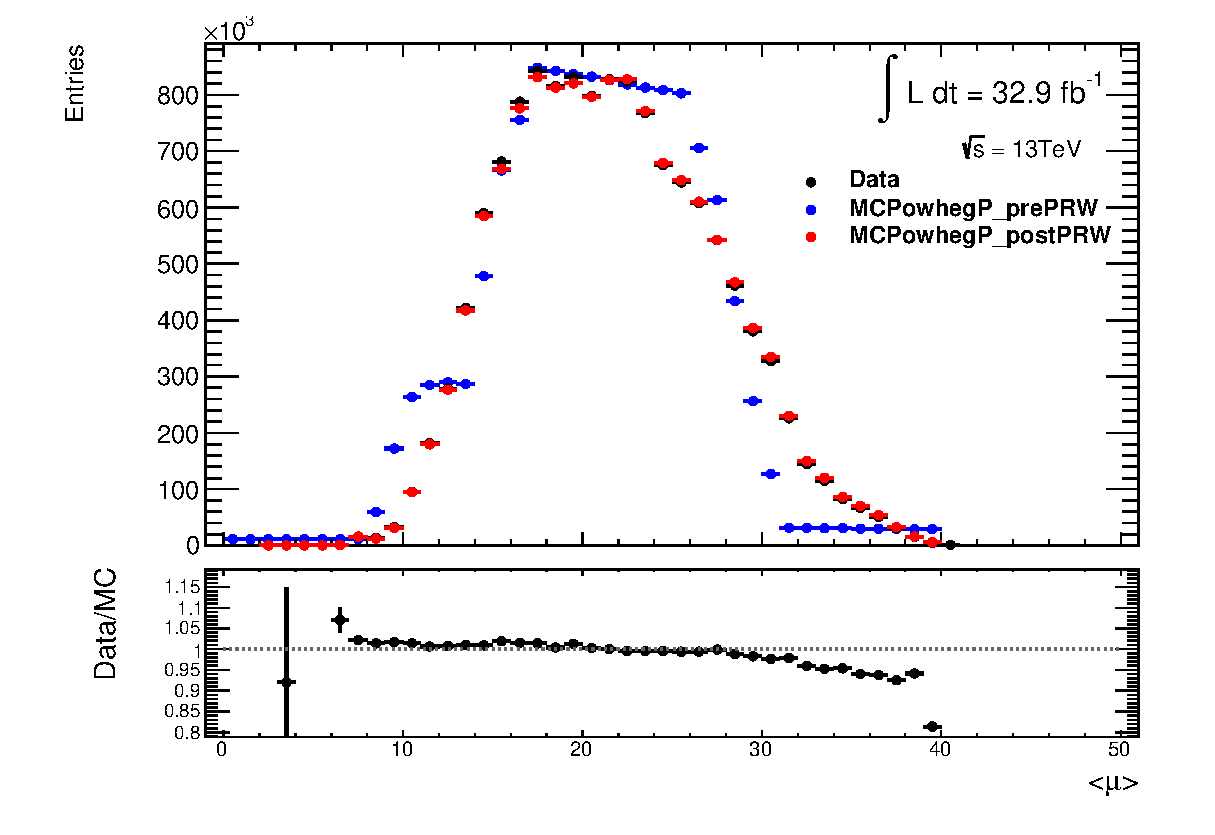
\includegraphics[width =0.9\linewidth]{images/Final_AvgMu}
    \caption{Distribución del número medio de interacciones por bunch crossing (luego de la selección de calidad de datos según la sección \ref{DataQu}) para colisiones $pp$ a $\sqrt{s}=$13TeV para datos recolectados en ATLAS durante 2016 a una luminosidad integrada de 32.9 $fb^{-1}$ (en negro), para la simulación nominal (Powheg $+$ Pythia) antes de la corrección de pile-up (en azul: ``MCPowhegP$\_$prePRW'') y para la simulación nominal luego de la correción de pile-up (en rojo:``MCPowhegP$\_$postPRW''). Algunos puntos negros quedan ocultos bajo puntos rojos. La distribución para los datos tiene una media $\overline{<\mu>}=$21.602$\pm$0.002 con una desviación estándar $\sigma=$5.673$\pm$0.001; y para la muestra simulada nominal luego de la corrección $\overline{<\mu>}=$21.672$\pm$0.001 y $\sigma=$5.709$\pm$0.001. En el panel inferior se puede ver el cociente de ambas distribuciones.}
    \label{fig:avgmu}
\end{figure}

\subsection{Calidad de Datos} \label{DataQu}

El primer paso en esta serie de selecciones tiene que ver con criterios de calidad que se aplican en datos (y cuando se indique también en MC) previo a cualquier recorte de índole cinemático. Estas recomendaciones se usan de base, con algunas excepciones, en todos los análisis de ATLAS y tienen que ver, principalmente, con el estado del detector. 

El primero de estos requerimientos de calidad es que el evento pertenezca a un LB que aparezca en la GRL\footnote{La GRL utilizada: data16$\_$13TeV.periodAllYear$\_$DetStatus-v88-pro20-21$\_$DQDefects-00-02-04$\_$PHYS$\_$StandardGRL$\_$All$\_$Good$\_$25ns.xml}.
Los LB son períodos de adquisición de datos de alrededor de uno o dos minutos, y varios cientos de LB se agrupan en $runs$.
Como ya se mencionó, un grupo encargado de estudiar la calidad de los datos adquiridos por el detector ATLAS produce una lista de aquellos LB registrados que son aptos para su uso en análisis físicos. Partiendo exclusivamente de aquellas runs\footnote{En esta tesis no se utiliza el dataset completo, es decir todas las runs registradas durante el año 2016, puesto que algunas runs serían enteramente descartadas por la GRL. Así, se decidió utilizar como dataset sólo aquellas runs que contengan algunos LB en la GRL.} con algún LB que figuren en la GRL, se tiene que la fracción de eventos considerados como ``buenos'' representa un $\sim 97\%$ de los eventos totales considerados.

El siguiente de los requerimientos tiene que ver con la reconstrucción de los vértices: se pide que en el evento haya al menos un vértice primario. Este criterio se aplica tanto en datos como en MC.

A continuación, en datos, evento a evento se buscan distintas \textit{flags} que alertan acerca del mal funcionamiento de algún sub-detector durante algún período de tiempo. En particular, se buscan flags en los calorímetros LAr, y los de tejas. Distintas señales abruptas y globales de ruido pueden aparecer en estos calorímetros en escalas temporales menores a las de un LB, con lo cual estos eventos no pueden ser excluidos por la GRL. Estos eventos son vetados en este paso.

%PODRIA PONER UN CUTFLOW DE ESTE CLEANING NOMAS..
%PORQUE SI PONGO CON TRIGGER TMB..->el trigger está preescaleado.


\subsection{Trigger}

Con la idea de seleccionar aquellos eventos de $Z\rightarrow \mu\mu$ se pide que los eventos pasen un $OR$ de dos triggers (a nivel HLT) que disparan ante muones, ambos alimentados por un trigger a nivel 1 (L1) del sistema de trigger de muones con umbral de 20GeV. El primero de ellos pide que haya al menos un muón en el evento, de calidad y aislación media con momento transverso por arriba de 26GeV. El segundo trigger considerado requiere que haya al menos un muón en el evento con $p_t>$50GeV.  
En la figura \ref{fig:trigEff} se muestra la eficiencia absoluta y relativa (al trigger L1 mencionado) del $OR$ de los triggers. 

\begin{figure}[ht]
    \centering
    \includegraphics[width =0.7\linewidth]{images/TriggEff1}
    \caption{Eficiencia del trigger de muones en función del $p_t$ del muón (reconstruido a nivel \textit{offline} usando software estándar de ATLAS) en la región del barril del detector. La eficiencia se determina en relación a muones aislados que pasan el criterio de calidad ``Media''. En negro se muestra la eficiencia absoluta del trigger a nivel 1 (L1) con umbral en 20GeV. En azul se muestra la eficiencia absoluta de un $OR$ de triggers que requieren al menos un muón de más de 26Gev y aislación media (determinada usando las trazas en el ID reconstruidas a nivel \textit{online} en el HLT) ó de más de 50GeV. En rojo se muestra la eficiencia de este trigger relativa a la curva negra. Esta eficiencia fue determinada usando el método de \textit{tag-and-probe} en candidatos a eventos de $Z\rightarrow \mu\mu$ (sin substracción de eventos de \textit{background}), en el que uno de los muones se utiliza para disparar el trigger y el otro para medir su eficiencia, en datos recolectados en 2016 a 13TeV. Sólo se muestran las incertezas estadísticas\cite{TrigEff} 
    }
    \label{fig:trigEff}
\end{figure}


Puede observarse que la combinación de triggers alcanza una eficiencia (relativa) cercana a 1 para muones con momento transverso superior a 26GeV.

A su vez, como en las simulaciones de MC resulta imposible tener en cuenta cada detalle del experimento real, cuestión que en última instancia también tiene efecto en la eficiencia del trigger en la simulación, el grupo de ``Muon Combined Performance'' (CP) dentro de ATLAS provee de un factor de corrección a la eficiencia del trigger simulado comparándola con la eficiencia del trigger que se tiene en los datos experimentales\cite{MCPGuidelines}. 

\subsection{Reconstrucción y selección de eventos}

El siguiente paso es la reconstrucción de los muones y los jets. Como ya se mencionó en la sección \ref{Muones}, los muones deben pasar ciertos criterios de calidad. Se seleccionan los eventos que tengan exactamente dos muones (\textit{combined}) de calidad \textit{Medium}\cite{SelTool}, aislados\cite{IsoTool} y con carga opuesta, ambos en el rango $|\eta|<$2.4 y $p_t>$25GeV. De la misma manera que con los triggers, el grupo CP provee de un factor de corrección \cite{MCPGuidelines} a aplicar en simulaciones de MC para dar cuenta de la diferencia entre la 
eficiencia de reconstrucción de los muones en datos experimentales y en las simulaciones. La forma en la que se determina la eficiencia de reconstrucción de los muones se explica en la referencia \cite{MuonReco}. 
\\

Los jets se reconstruyen utilizando el algoritmo anti-$k_t$ a partir de la escala EM para los Ref Jets, y a partir de la escala LCW para los R-scan Jets. Esto quiere decir que en un mismo evento los jets se reconstruyen de tres maneras diferentes ($R=$0.4, 0.2 y 0.6 respectivamente). Las colecciones de jets se calibran evento a evento como ya fue explicado en \ref{Rscan}. En una primera instancia, se rechazan todos los jets con $|y|>$4.4 y los que se encuentren a una distancia angular $\Delta R<$0.35 de cualquiera de los dos muones. 

Además, los eventos también se evalúan considerando la \textit{calidad} de los jets, criterio que se aplica tanto en datos como en MC. Cuando se reconstruyen los eventos, es posible que jets formados con información de los calorímetros sean generados por fuentes \footnote{Por ejemplo, ruido abrupto en el calorímetro, rayos cósmicos u otros backgrounds que no provienen de la colisión.} que nada tienen que ver con el flujo de energía desde el hard scatter. Entonces, la referencia \cite{JetCleaning} propone dos selecciones para identificar estos jets falsos: ``BadLoose'' y ``BadTight'', que tienen en cuenta distintos cocientes de energía (por ejemplo, los cocientes entre la energía depositada en el calorímetro EM o hadrónico y la energía total del jet) y variables que consideran las trazas que dan origen a ese jet (por ejemplo, el cociente entre la suma escalar del $p_t$ de las trazas con origen en el vértice primario y el momento del jet). La primera es la que se usa en este trabajo y  está diseñada para mantener alta la eficiencia de jets ``buenos'' manteniendo la eficiencia de rechazo a los jets falsos lo más alta posible. La estrategia de selección de eventos debido a estos criterios de calidad sobre los jets se aplica solamente a los Ref Jets según las recomendaciones en \cite{JetCleaningTool}, en las que se busca descartar aquellos eventos que tengan algún Ref Jet de tipo ``LooseBad'' pero que no hayan sido etiquetados como pile-up jets. Una cantidad que se utiliza para discriminar jets provenientes del hard scatter de pile-up jets es el coeficiente de \textit{Jet Vertex Tagger} o JVT, el cual pide a los jets con $p_t<$50GeV y $|\eta|<$2.4 que estén asociados con un vértice primario (al \textit{working point} medio de JVT \cite{JVTtool}), identificando el 92$\%$ de hard-scatter jets y el $98\%$ de pile-up jets. La selección de eventos debido a la calidad de los jets entonces descarta aquellos eventos con ``LooseBad'' jets que estén fuera del rango de aplicación del criterio de JVT, y aquellos con ``LooseBad'' jets que JVT identifique como provenientes del hard-scatter. \\ 


\begin{figure}[ht]
    \centering
    \begin{subfigure}[b]{0.495\textwidth}
        \centering
        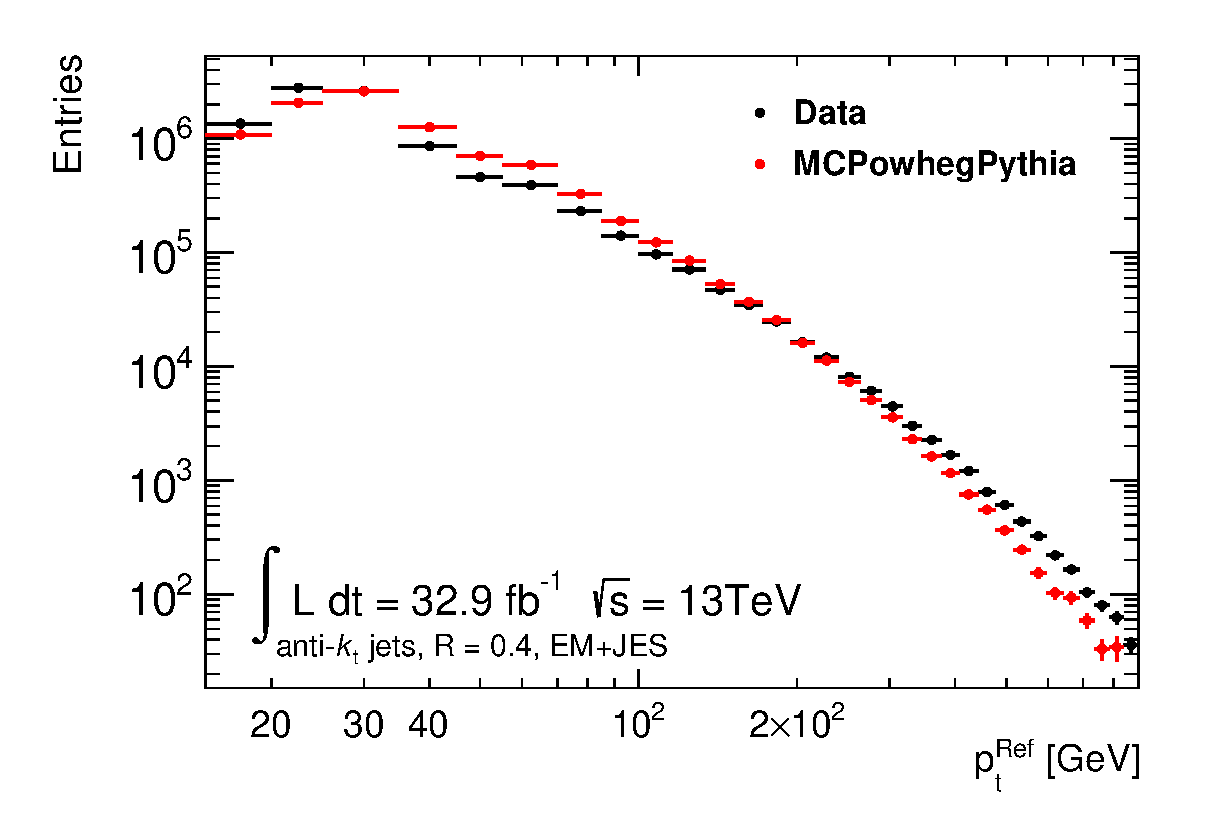
\includegraphics[width=\textwidth]{images/Final_LeadRefPt}
        \caption{ }
        \label{fig:JetptDist}
    \end{subfigure}
    \hfill
    \begin{subfigure}[b]{0.495\textwidth}
        \centering
        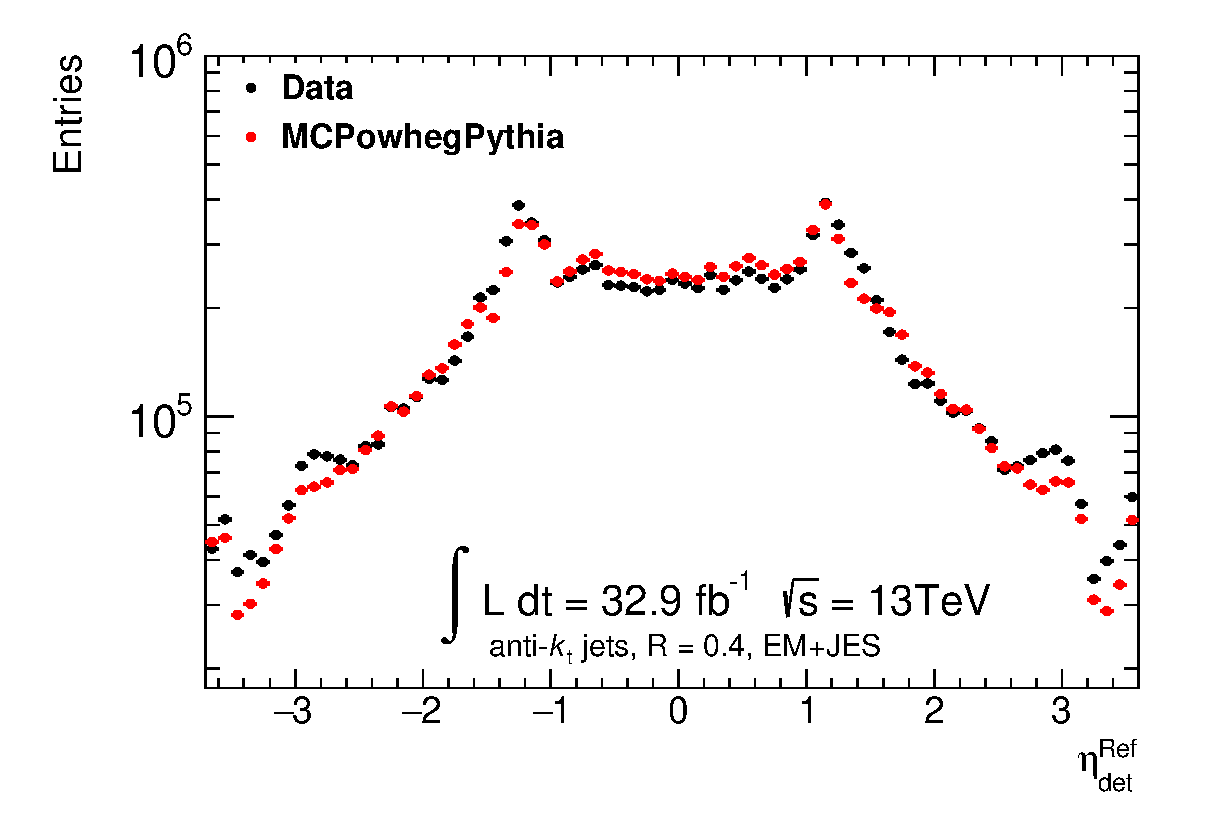
\includegraphics[width=\textwidth]{images/Final_RefLeadEta}
        \caption{}
        \label{fig:JetEtaDist}
    \end{subfigure}
    \caption{ Distribución de (a) $p_t^{Ref}$ y (b) $\eta_{det}^{Ref}$ para datos recolectados en ATLAS en 2016 (en negro) y para la muestra nominal de MC (en rojo), luego de la selección inicial de eventos.}
    \label{fig:JetDistro}
\end{figure}

En la figura \ref{fig:JetDistro} se muestra la distribución del momento transverso del Ref Jet con mayor momento, o \textit{leading} jet, y la distribución de pseudo-rapidez. En ambos casos se muestran las distribuciones tanto en datos como en la muestra nominal de MC.\\ 

El siguiente paso de la selección tiene que ver con seleccionar los eventos que contengan un candidato a $Z$. Para ello se calcula la masa invariante de los dos muones y se seleccionan aquellos eventos tal que la misma sea consistente con la masa de un $Z$: 80GeV$<m_{\mu \mu}<$116GeV. En la figura \ref{fig:Zmass} puede verse la distribución de la masa invariante de los dos muones tanto en datos como en MC. Se observa que la simulación reproduce la forma de la distribución en datos, mostrando una resonancia acorde con un $Z$; y en la figura \ref{fig:Zpt} puede verse la distribución de $p_t$ del $Z$ reconstruido para los eventos seleccionados. 

\begin{figure}[ht]
    \centering
    \begin{subfigure}[b]{0.495\textwidth}
        \centering
        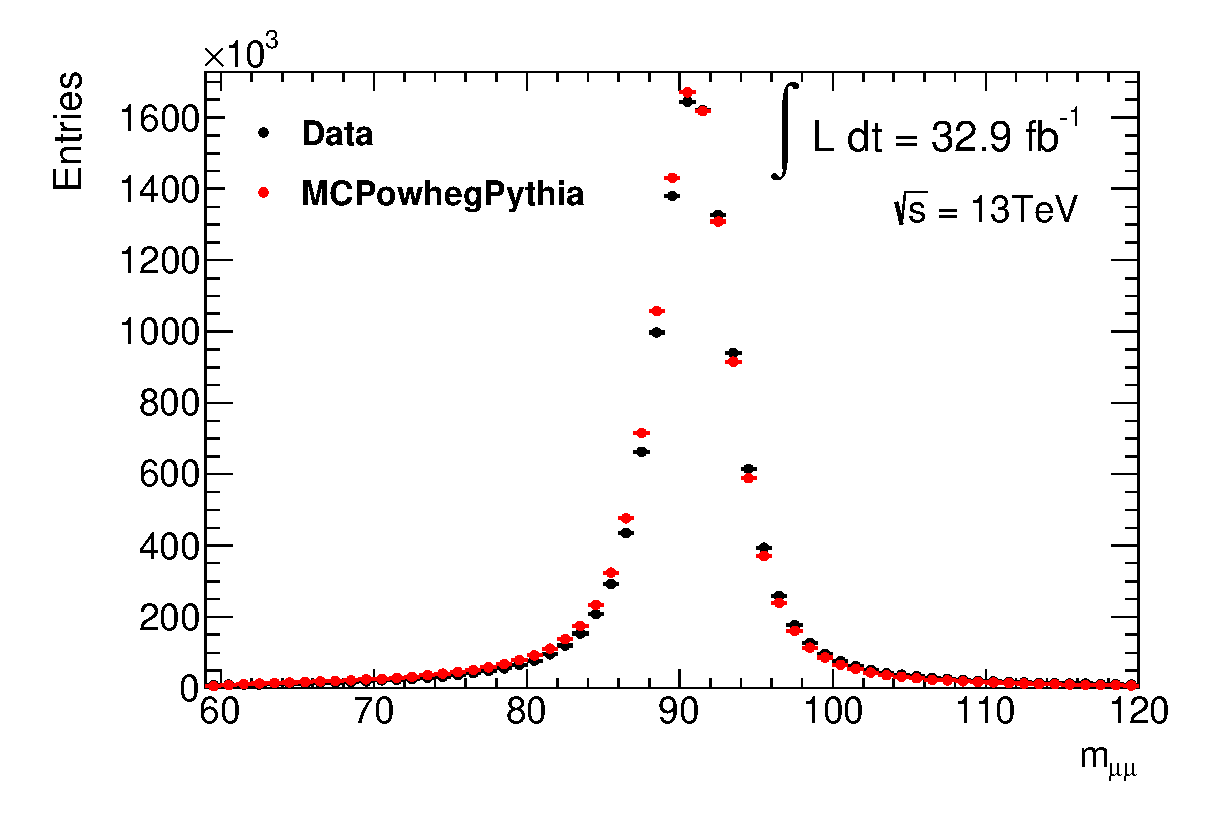
\includegraphics[width=\textwidth]{images/Final_Zmass}
        \caption{}
        \label{fig:Zmass}
    \end{subfigure}
    \hfill
    \begin{subfigure}[b]{0.495\textwidth}
        \centering
        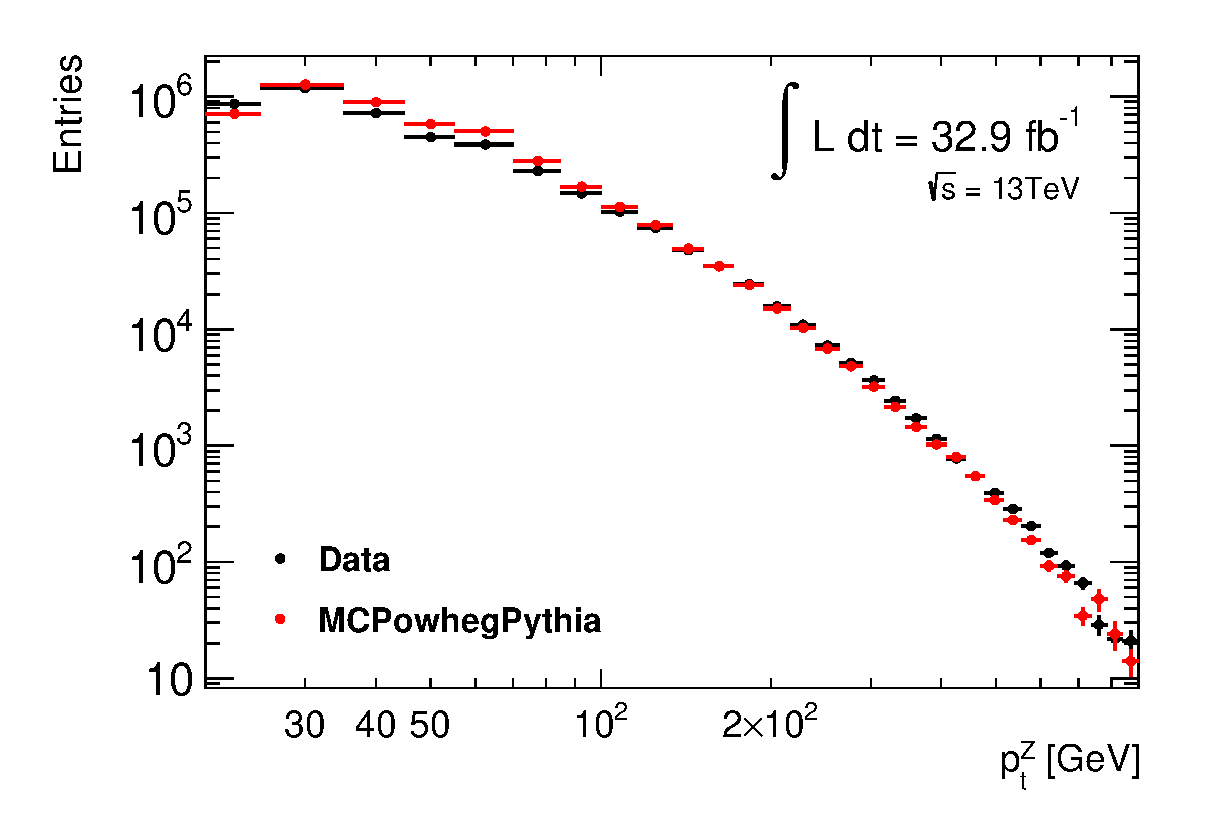
\includegraphics[width=\textwidth]{images/Final_Zpt}
        \caption{}
        \label{fig:Zpt}
    \end{subfigure}
    \caption{ En negro se muestra la distribución correspondiente a los datos recolectados en ATLAS en 2016, aprobados por la GRL, y en rojo se muestra la distribución correspondiente a la muestra de MC nominal (Powheg + Pythia) para (a) la masa invariante del par de muones para los eventos seleccionados, y (b) el $p_t^Z$ resultante luego de la selección de eventos con masa invariante del par de muones consistente con la masa del Z.} 
    \label{fig:Z}
\end{figure}

Finalmente, se descartan aquellos eventos que luego de estos recortes no contengan al menos un R-scan Jet y al menos un Ref Jet.

\subsection{Selección de Jets}

El primer paso para derivar la calibración R-scan es calcular el cociente $\mathcal{R}$. El estudio se realiza primero para la colección de R-scan Jets con un $R$ y luego se repite el procedimiento para el otro. Para poder calcular este cociente primero se requiere de una selección de los jets a utilizar. En la tabla \ref{tab:sel} se resumen los distintos cortes aplicados a las colecciones de jets, indicando su valor nominal, y su variación sistemática cuando corresponda (ver sección \ref{Syst}).

\begin{table}[ht]
    \centering
    \begin{tabular}{|l|l|l|} 
        \hline
        %\multicolumn{2}{|c|}{input} & \multicolumn{2}{c|}{output} & \\
        Selección & Valor Nominal & Variación Sistemática\\ \hline\hline
        Ref Jet $p_t$  & $>15$GeV &\\ \hline
        Ref Jet $\eta$ & $|\eta|<$3 & \\ \hline
        Rscan Jet $p_t$ & $>10$GeV &  \\ \hline
        Rscan Jet $\eta$ & $|\eta|<$3 & \\ \hline
        $\Delta \varphi (Z,jet^{Ref})$ & $|\Delta\varphi|>$1.57 &\\ \hline
        Aislación $\Delta R> f*R$ & $f=2$ & 1.5 ($\downarrow$) 2.5 ($\uparrow$) \\ \hline
        $p_{t,\%}$ & 10 $\%$ & 5$\%$ ($\downarrow$) $20\%$($\uparrow$)  \\ \hline
        JVT & 0.59 & 0.11 ($\downarrow$) 0.91 ($\uparrow$) \\ \hline
        Matching $\Delta R(jet^{Rscan},jet^{Ref})<dR$ & 0.2 & 0.1 ($\downarrow$) 0.3 ($\uparrow$)\\ \hline
    \end{tabular}
    \caption{Resumen de cortes aplicados a los jets durante el proceso de selección en el método de direct-matching para eventos de $Z+jets$.}
    \label{tab:sel}
\end{table}


Como primera medida, se seleccionan los Ref Jets con $p_t>$15GeV, ya que para valores inferiores la JES no está bien definida y, por lo tanto, no se puede decir que el Ref Jet esté bien calibrado como para servir de objeto de referencia para calibrar los R-scan Jets; y que se encuentren en el hemisferio opuesto al Z pidiendo $|\Delta \varphi|>$1.57; y los R-scan con $p_t>$10GeV. Además, se pide que ambos tipos de jets estén en la región $|\eta^{det}|<$3 con la intención de evitar posibles sesgos provenientes del hecho de que el trigger de muones está limitado a $|\eta|<$2.4.\\

%y Ref Jets con eta menor a 3.0 por fisica: para no introducir un bias con Z forward-> mi trigger de muones solo anda en eta central y porque no se necesita estudiar el caso forward

\noindent \textbf{Aislación}:

\indent La calibración dada por este método tiene sentido cuando se trata de jets aislados, de otra forma no se podría hallar una correspondencia entre el R-scan Jet que se identifica angularmente con un Ref Jet. Por ejemplo, podría tenerse el caso en que un R-scan Jet de $R=$0.6 englobe parte de dos Ref Jets. En estos casos, resultaría incorrecto asumir que el $p_t$ de uno de los Ref Jets sirve como referencia para calibrar el momento del R-scan Jet. El criterio de aislación aplicado utiliza distinto umbral cuando se trata de pedir aislación para RefJet-RefJet y RscanJet-RscanJet, ya que tiene en cuenta que justamente los jets tienen distinto tamaño. Entonces, se guardan aquellos jets que verifican $\Delta R >f*R$, donde $\Delta R$ se calcula entre jets de la misma colección, $R$ es el radio de la colección, y $f$ un factor, que en el caso nominal vale 2, que determina qué tan separados deben estar los centros de los jets en  unidades de $R$. Como el discriminante se calcula de a pares de jets, no se descartan automáticamente ambos jets si resultara que no están aislados, sino que se tiene en cuenta la relación entre los momentos de ambos jets. Es decir, se descarta el de menor momento ($p_{t,1}$), y para decidir sobre el de mayor momento($p_{t,2}$) se tiene en cuenta qué porcentaje, ($p_{t_{\%}}$), representa el momento del primero con respecto al segundo, descartándose si $p_{t,1}> p_{t_{\%}}*p_{t,2}$. \\

\noindent \textbf{Matching}:

El último paso de esta serie de selecciones es identificar (\textit{matching}) en el evento un Ref Jet con un R-scan Jet. Para ello, se calcula la distancia angular de un Ref Jet a todos los R-scan Jets y se conserva el par de menor $\Delta R$. Si esta distancia es tal que $\Delta R < dR$ se dice que Ref Jet y R-scan Jet se corresponden y se toma entre ellos el cociente $\mathcal{R}$, y ambos jets se retiran de la lista de jets disponibles para realizar el \textit{matching}. En este proceso sólo se utilizan Ref Jets que no hayan sido identificados como pile-up jets por el criterio de JVT (o que estén en el rango en el que no se aplica el criterio). Los valores de $\mathcal{R}$ obtenidos se organizan en bines de $\eta^{Rscan}_{det}$ y $p_t^{Rscan}$. Debido a que la estadística lo permite se trata de hacer un bineado fino (en pasos de 0.1) en $\eta$ para dar poder relacionar la dependencia de esta variable con los distintos sectores y tecnologías del detector. 

En la figura \ref{fig:ResponseTH2} se muestran dos histogramas de $\mathcal{R}$ en función de $p_t^{Rscan}$ para un dado bin de $\eta^{Rscan}_{det}$ para los dos radios de Rscan Jets estudiados.

\begin{table}[ht]
    \centering
    \begin{tabular}{|l|l|l|l|l|} 
        \hline
        %\multicolumn{2}{|c|}{input} & \multicolumn{2}{c|}{output} & \\
        Corte & Datos & Datos($\%$) & MC & MC ($\%$) \\ \hline\hline
        Total & 60969945 & 100$\%$ & 36270278 & 100$\%$ \\ \hline
        \textbf{Cortes de calidad} & & & &\\ 
        GRL   & 59427896 & 97.5$\%$ & 36270278 & 100$\%$  \\
        Flags / 1 NPV & 59328706 & 97.3$\%$ & 36270265 & 99.99$\%$ \\\hline
        \textbf{Z+jets} & & & &  \\ 
        Trigger & 22949389 & 37.6$\%$ & 32383140 & 89.3$\%$ \\ 
        2 Muones & 13185100 & 21.6$\%$ & 21603561 & 59.7$\%$\\
        Carga Opuesta & 13182303 & 21.6$\%$ & 21603430 & 59.7$\%$\\
        $m_{\mu\mu}$ & 12125856 & 19.9$\%$ & 20119367 & 55.5$\%$\\ \hline
        \textbf{Direct-Matching} & & & & \\ 
        1 Ref/1 Rscan & 11104767 & 18.2$\%$ & 18762764 & 51.7$\%$ \\
        JetCleaning & 10941998 & 17.9$\%$ & 8362403 & 23.1$\%$ \\ 
        $\Delta \phi$ & 9596352 & 15.7$\%$ & 7141075 & 19.7$\%$ \\
        Matching  & 4147037 & 6.8$\%$ & 3950267 & 10.9$\%$ \\ \hline 
        \end{tabular}
    \caption{\textit{Cutflow} de selección de eventos en datos y en la muestra nominal de MC utilizada, Powheg+Pythia.}
    \label{tab:cut}
\end{table}


\begin{figure}[ht]
    \centering
    \begin{subfigure}[b]{0.495\textwidth}
        \centering
        \includegraphics[width=\textwidth]{images/Th2_Data_2lc_eta49}
        \caption{}
        %\label{fig:Th22lc}
    \end{subfigure}
    \hfill
    \begin{subfigure}[b]{0.495\textwidth}
        \centering
        \includegraphics[width=\textwidth]{images/Th2_data_6lc_eta49}
        \caption{}
        %\label{fig:Th26lc}
    \end{subfigure}
    \vfill
    \begin{subfigure}[b]{0.495\textwidth}
        \centering
        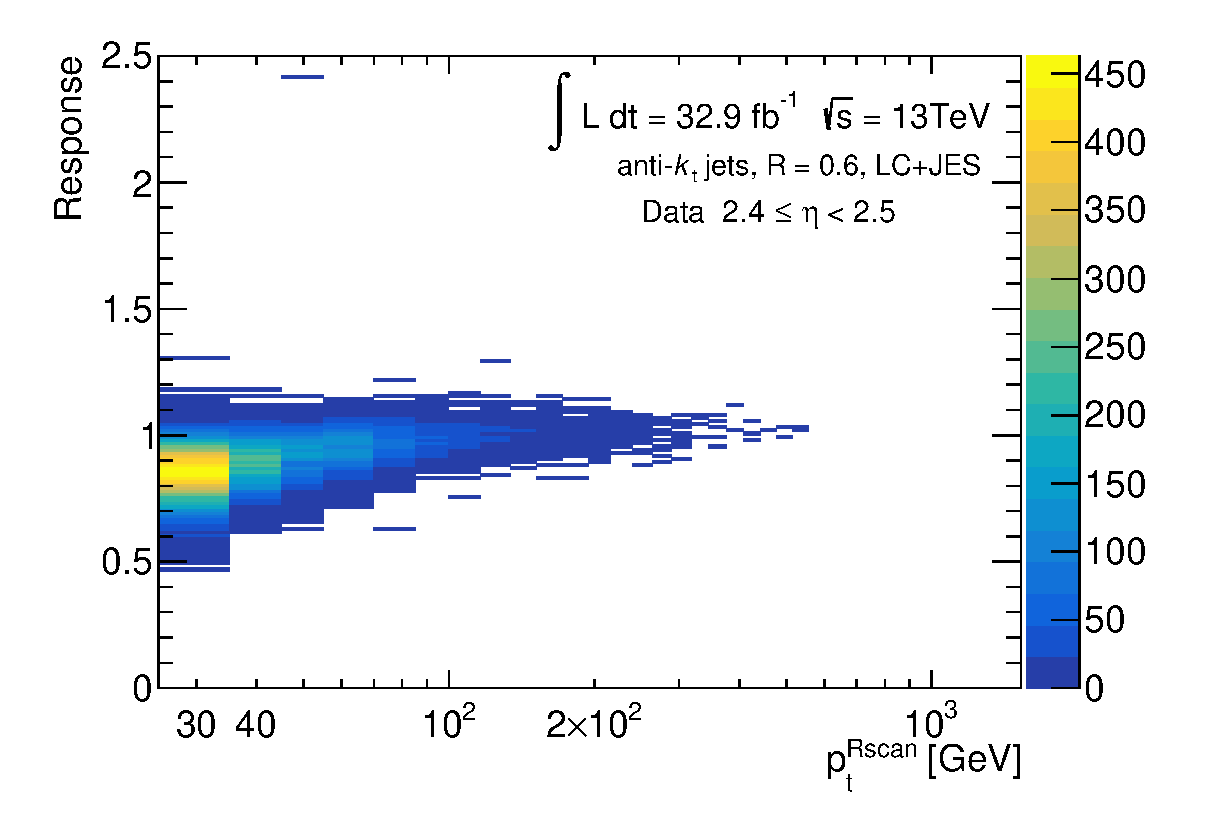
\includegraphics[width=\textwidth]{images/Th2_Data_2lc_eta69}
        \caption{}
        %\label{fig:Th26lc}
    \end{subfigure}
    \hfill
    \begin{subfigure}[b]{0.495\textwidth}
        \centering
        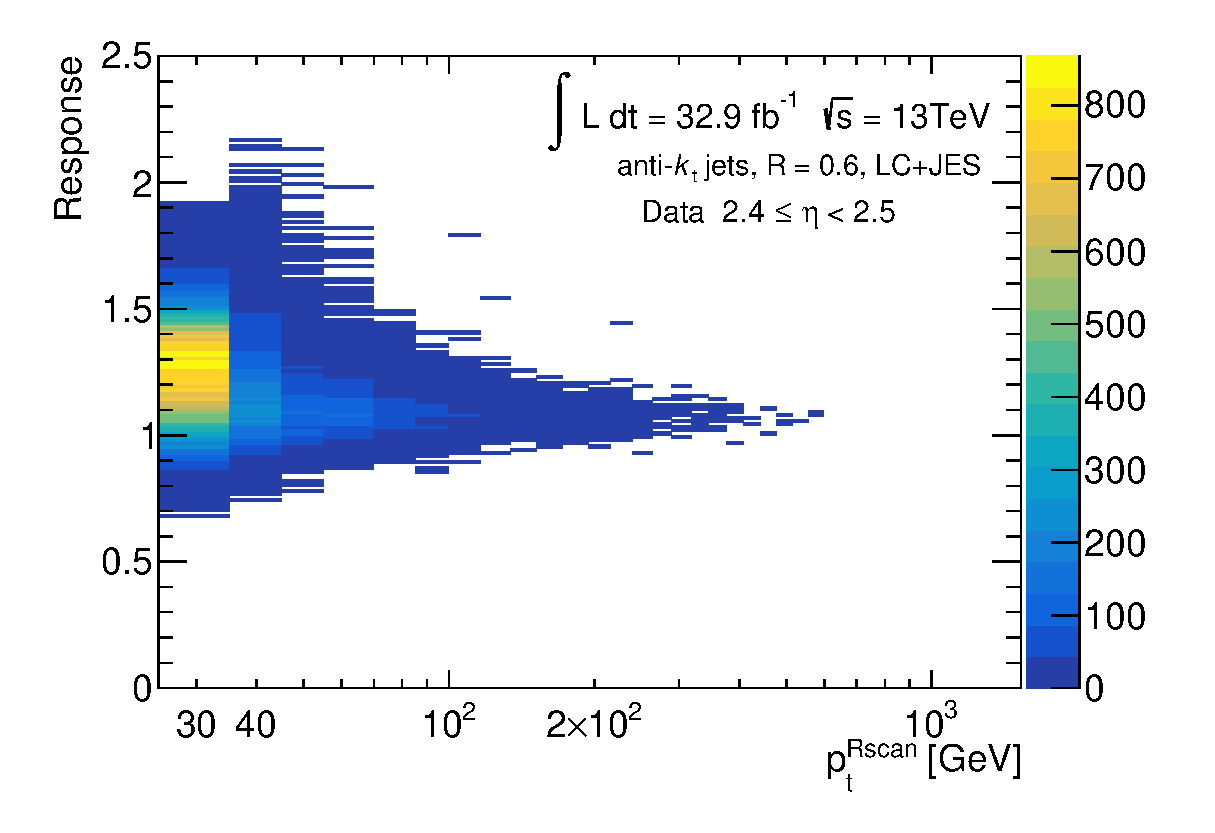
\includegraphics[width=\textwidth]{images/Th2_data_6lc_eta69}
        \caption{}
        %\label{fig:Th26lc}
    \end{subfigure}
    \caption{Distribuciones de la \textit{response} ($\mathcal{R}$) para el bin 0.4$<\eta^{Rscan}_{det}<$0.5 para la colección Rscan con (a) $R_{rscan}=$0.2 y (b) $R_{rscan}=$0.6, y para el bin 2.4$<\eta^{Rscan}_{det}<$2.5 para (c) $R_{rscan}=$0.2 y (d) $R_{rscan}=$0.6 en función de $p_t^{Rscan}$ para el bin de 2.4$<\eta^{Rscan}_{det}<$2.5, en datos recolectados en ATLAS en 2016. La escala de colores da cuenta de las entradas en cada bin.} 
    \label{fig:ResponseTH2}
\end{figure}

\subsection{Análisis}
En los gráficos en la figura \ref{fig:ResponseTH2} se observan algunas tendencias que se repiten tanto en datos como en la simulación y para todos los rangos de $\eta$. La primera a mencionar es que en todos los casos, datos y MC y ambas colecciones de Rscan Jets, la estadística es mayor a bajo momento, siendo máxima en el bin 15 GeV$<p_t^{Rscan}<$20 GeV en el caso de la colección de $R=$0.2 y en el bin  25 GeV$<p_t^{Rscan}<$35 GeV en el caso de la colección de $R=$0.6, y disminuye a medida que aumenta el momento del Rscan Jet. Además, a medida que aumenta el momento del Rscan Jet se observa también que la dispersión de los datos se reduce, y el $\mathcal{R}$ tiende a uno, por valores de $\mathcal{R}$ inferiores para el caso de la colección 0.2 y por encima para el caso de la colección 0.6.
\begin{figure}[ht]
    \centering
    \begin{subfigure}[b]{0.495\textwidth}
        \centering
        \includegraphics[width=\textwidth]{images/Data_2lc_49}
        \caption{Datos}
        %\label{fig:data2lc49}
    \end{subfigure}
    \hfill
    \begin{subfigure}[b]{0.495\textwidth}
        \centering
        \includegraphics[width=\textwidth]{images/MC_2lc_49}
        \caption{MC Powheg+Pythia}
        %\label{fig:Th26lc}
    \end{subfigure}
    \vfill
    \begin{subfigure}[b]{0.495\textwidth}
        \centering
        \includegraphics[width=\textwidth]{images/Data_6lc_49}
        \caption{Datos}
        %\label{fig:Th26lc}
    \end{subfigure}
    \hfill
    \begin{subfigure}[b]{0.495\textwidth}
        \centering
        \includegraphics[width=\textwidth]{images/MC_6lc_49}
        \caption{MC Powheg+Pythia}
        %\label{fig:Th26lc}
    \end{subfigure}
    \caption{ Se muestran los histogramas de \textit{response} y su correspondiente ajuste Gaussiano, indicando con una línea rellena el rango utilizado en el ajuste. Todos los histogramas corresponden al bin 0.4$<\eta^{Rscan}_{det}<$0.5. En el panel superior se muestra el bin 20 GeV$<p_t^{Rscan}<$25 GeV para la colección Rscan con $R_{rscan}=$0.2 en (a) datos de ATLAS 2016 y (b) MC Powheg+Pythia. En el panel inferior se muestra el bin 45 GeV$<p_t^{Rscan}<$55 GeV (c) $R_{rscan}=$0.2 y (d) $R_{rscan}=$0.6 en función de $p_t^{Rscan}$ para la colección con $R_{rscan}=$0.6 en (c) Datos de ATLAS 2016 y (d) MC Powheg+Pythia.} 
    \label{fig:Fits}
\end{figure}

El resto del proceso para derivar la calibración básicamente depende de estos histogramas bidimensionales (y para cada $\eta^{Rscan}_{det}$). Para obtener una calibración (también) en función de $p_t^{Rscan}$, estos histogramas se proyectan en los diferentes bines de $p_t$, obteniéndose histogramas de $\mathcal{R}$ (\textit{response}) para cada bin de $p_t^{Rscan}$ y $\eta_{det}^{Rscan}$. Si bien las distribuciones de \textit{Response} resultan asimétricas, los ajustes gaussianos realizados describen apropiadamente el ``core'' de las distribuciones. En la figura \ref{fig:Fits} se observan algunas distribuciones de $\mathcal{R}$ para un mismo $\eta$ bin tanto, datos como en MC, para ambas colecciones de Rscan Jets. La asimetría mencionada es más pronunciada en el caso de los Rscan Jets con $R=$0.6 en los bines de bajo momento, como se ejemplifica en el panel inferior de la figura \ref{fig:Fits} tanto en datos y en MC. En estas situaciones, se prestó cuidadosa atención a que el ajuste Gaussiano realizado representara adecuadamente el centro de la distribución. En general, la estadística obtenida en las muestras permitió realizar buenos ajustes a partir de $p_t^{Rscan}>$15GeV ($p_t^{Rscan}>$25GeV) y hasta $p_t^{Rscan}\sim$300GeV en la región central $|\eta_{det}^{Rscan}|<$2, disminuyendo el rango hasta $p_t^{Rscan}\sim$200GeV en la región 2$<|\eta_{det}^{Rscan}|<$3, tanto en datos y MC para la colección 0.2 (0.6).  


Con el valor medio que provee el ajuste se mide $<\mathcal{R}>$ en función de $p_t^{Rscan}$ tanto en datos como en MC, para todos los bines de $\eta$ y para ambas colecciones. Finalmente, para cada bin de $\eta$ se toma el cociente entre MC y datos para obtener la corrección ($\mathcal{C}$) a aplicar en los datos. En la figura \ref{fig:Response} se ejemplifica para ambas colecciones de Rscan Jets en los bines 0.4$<\eta^{Rscan}_{det}<$0.5 y 2.4$<\eta^{Rscan}_{det}<$2.5. El error estadístico asociado al valor medio de la response en cada bin corresponde al error con el que el ajuste estima el valor medio de la Gaussiana, y el error en $\mathcal{C}$ resulta de propagar los errores anteriores. 
\begin{figure}[ht]
    \centering
    \begin{subfigure}[b]{0.495\textwidth}
        \centering
        \includegraphics[width=\textwidth]{images/ResponseRatio2LC_49}
        \caption{$R=$0.2 ; 0.4$<\eta^{Rscan}_{det}<$0.5}
        %\label{fig:data2lc49}
    \end{subfigure}
    \hfill
    \begin{subfigure}[b]{0.495\textwidth}
        \centering
        \includegraphics[width=\textwidth]{images/ResponseRatio2LC_69}
        \caption{$R=$0.2 ; 2.4$<\eta^{Rscan}_{det}<$2.5}
        %\label{fig:Th26lc}
    \end{subfigure}
    \vfill
    \begin{subfigure}[b]{0.495\textwidth}
        \centering
        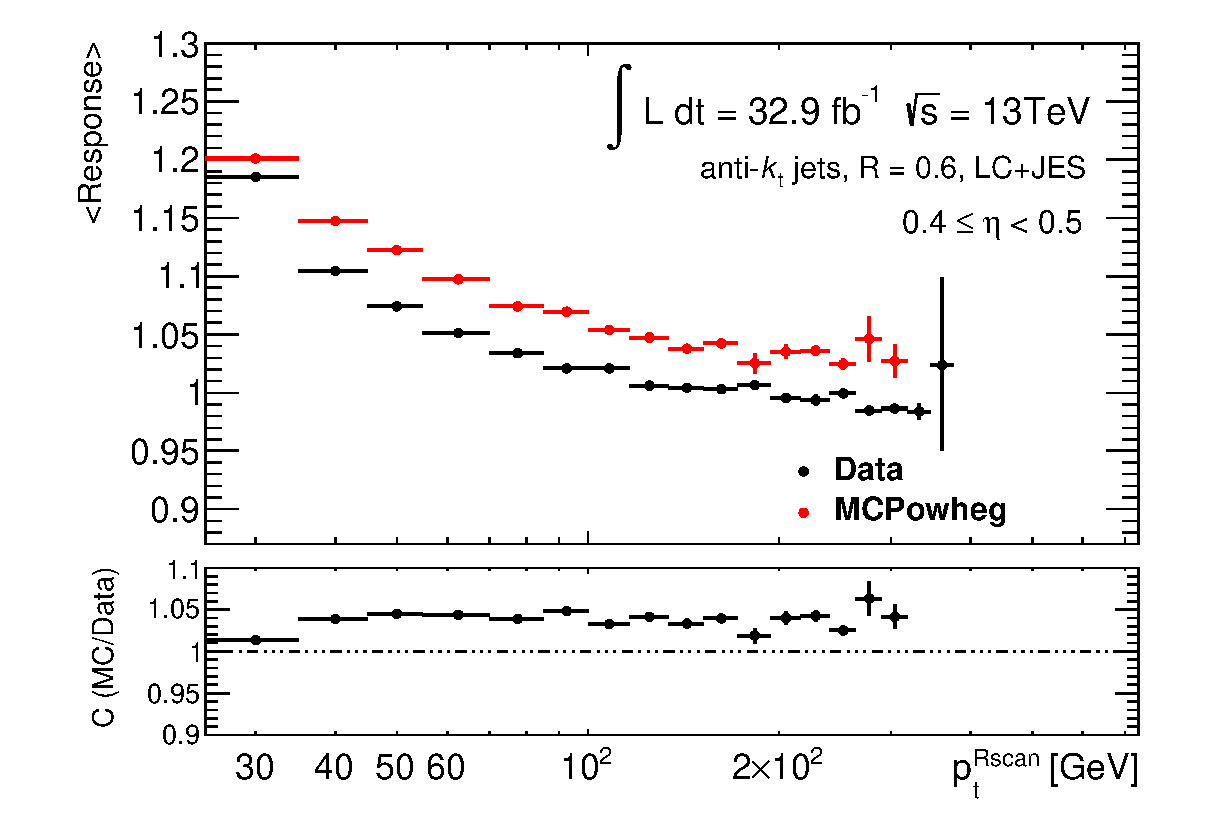
\includegraphics[width=\textwidth]{images/ResponseRatio6LC_49}
        \caption{$R=$0.6 ; 0.4$<\eta^{Rscan}_{det}<$0.5}
        \label{fig:fitFeo}
    \end{subfigure}
    \hfill
    \begin{subfigure}[b]{0.495\textwidth}
        \centering
        \includegraphics[width=\textwidth]{images/ResponseRatio6LC_69}
        \caption{$R=$0.6 ; 2.4$<\eta^{Rscan}_{det}<$2.5}
        %\label{fig:Th26lc}
    \end{subfigure}
    \caption{ Paneles superiores: gráfico del valor medio $<\mathcal{R}>$ en función de $p_t^{Rscan}$ para datos (en negro) recolectados en ATLAS en 2016 y para la muestra nominal, Powheg+Pythia, de MC (en rojo). Paneles inferiores: cociente entre MC y Datos.} 
    \label{fig:Response}
\end{figure}


En la figura \ref{fig:Response} puede observarse una tendencia característica, al igual que en la figura \ref{fig:ResponseTH2}: a medida que aumenta $p_t^{Rscan}$ se observa que $<\mathcal{R}>$ en cada caso comienza a tender hacia un valor estable, por debajo en el caso $R=$0.2, y por encima en el caso $R=$0.6. Observar este crecimiento (decrecimiento) de $<\mathcal{R}>$ en el caso de Rscan Jets con $R=$0.2 (0.6) en datos y MC, pero sobre todo en MC, sugiere que la diferencia en tamaño es la causa. Es decir, en MC los Rscan Jets y los Ref Jets están, prácticamente, calibrados al mismo nivel (no así en datos), por lo que este comportamiento de la response se debe exclusivamente al hecho de haber calibrado los jets con distinto tamaño. Esta tendencia observada en jets aislados podría asociarse con el hecho de que a bajo momento la lluvia de partículas es más ancha y, por lo tanto, al reconstruirla con un jet de radio menor el algoritmo forma el jet de manera diferente y con una menor cantidad de celdas calorimétricas que con un radio mayor, perdiéndose información y reconstruyendo un momento menor en relación al caso de radio mayor.

Además, la tendencia observada en la figura \ref{fig:Response} (y en todos los bines de $\eta$ estudiados) es suave salvo en los últimos bines de momento alcanzados, consistente con el hecho de que a bajo momento se tiene una cantidad de estadística considerablemente mayor, lo que permite hacer un bineado fino en las distribuciones de $\mathcal{R}$ dando más puntos como input al ajuste del core. 

La presencia de algunos puntos con error considerablemente mayor al resto, y desviados de la tendencia general en los gráficos de $\mathcal{R}$, como se ejemplifica en la figura \ref{fig:fitFeo}, se debe, principalmente, a la estadística. Los ajustes gaussianos se realizan de manera automatizada ya que se deben ajustar para cada uno de los 60 bines de $\eta$ más de 30 bines de $p_t$, y esto realizarlo en datos y en MC, y para ambas colecciones de Rscan Jets. Para implementar la automatización, sobre una misma distribución se realizan varios ajustes variando el rango y se toma el mejor ajuste en el sentido de $\chi^2$, pero, a veces, los ajustes que se obtienen no representan adecuadamente a las distribuciones. Por ejemplo, en la figura \ref{fig:DistroFitMalo} se muestra el bin correspondiente 0.4$<\eta^{Rscan}_{det}<$0.5 y 346 GeV$<p^{Rscan}_{t}<$376 GeV para la colección $R=$0.6 en datos, correspondiente a la figura \ref{fig:fitFeo}. Esta figura ejemplifica un caso en el que variar el rango del ajuste, se tiene una mejor calidad en el sentido de $\chi^2$, pero el valor medio obtenido, o mejor dicho el ajuste, no describe apropiadamente la distribución, con lo cual no se debería tener en cuenta ese punto.


\begin{figure}[ht]
    \centering
    \includegraphics[width =0.7\linewidth]{images/FitMalo}
    \caption{Distribución de la response en el bin de 0.4$<\eta^{Rscan}_{det}<$0.5 y 346GeV$<p^{Rscan}_{t}<$376GeV para datos recolectados en ATLAS en 2016. La línea dibujada representa la curva ajustada, la parte rellena indica el rango utilizado para realizar el ajuste Gaussiano. En el rango seleccionado, la curva pasa directamente por los datos, dando un $\chi^2=$0; sin embargo, el ajuste realizado no es representativo de la distribución.}
    \label{fig:DistroFitMalo}
\end{figure}

Las distribuciones de $\mathcal{R}$ obtenidas para datos y la muestra nominal de Powheg+Pythia, en general, tienen buena estadística en el rango de momentos considerado, con lo cual este tipo de fallas rara vez sucede, y cuando sucede lo hace llegando al extremo superior del rango, nuevamente, donde la estadística es menor.\\ 

En el estudio del error sistemático asociado a la elección de un generador de MC se debió trabajar con otra muestra de MC, generada usando \textit{Sherpa} como fue mencionado en la sección \ref{Muestras}. Al repetir este procedimiento utilizando esta muestra se observa que la estadística en las distribuciones de $\mathcal{R}$ es baja en el rango en el que se quiere derivar la calibración. Esto se evidencia en los gráficos de $<\mathcal{R}>$ en función del momento al notar una mayor dispersión de los puntos respecto de la tendencia general observada. Este comportamiento se debe principalmente a que la estadística registrada es mucho menor, en todo el rango de momento estudiado. Esto trae como consecuencia una mayor cantidad de ajustes malos, que ocurren ya en todo el rango y no sólo en el extremo superior como era el caso de datos y Powheg+Pythia, y que deben ser repetidos o estudiados uno por uno. Además, los puntos utilizados para realizar el ajuste tienen asociados un error estadístico mayor. Entonces, de cierta manera, varias curvas pueden ajustar dichos puntos, y por lo tanto, el $<\mathcal{R}>$ se estima con un error mayor. En la figura \ref{fig:ResponseSherpa} se muestran los mismos gráficos que en la figura \ref{fig:Response} pero para el caso en que la muestra de MC corresponde al generador Sherpa.\\    

\begin{figure}[ht]
    \centering
    \begin{subfigure}[b]{0.495\textwidth}
        \centering
        \includegraphics[width=\textwidth]{images/ResponseRatio2LC_49_Sherpa}
        \caption{$R=$0.2 ; 0.4$<\eta^{Rscan}_{det}<$0.5}
        %\label{fig:data2lc49}
    \end{subfigure}
    \hfill
    \begin{subfigure}[b]{0.495\textwidth}
        \centering
        \includegraphics[width=\textwidth]{images/ResponseRatio2LC_69_Sherpa}
        \caption{$R=$0.2 ; 2.4$<\eta^{Rscan}_{det}<$2.5}
        %\label{fig:Th26lc}
    \end{subfigure}
    \vfill
    \begin{subfigure}[b]{0.495\textwidth}
        \centering
        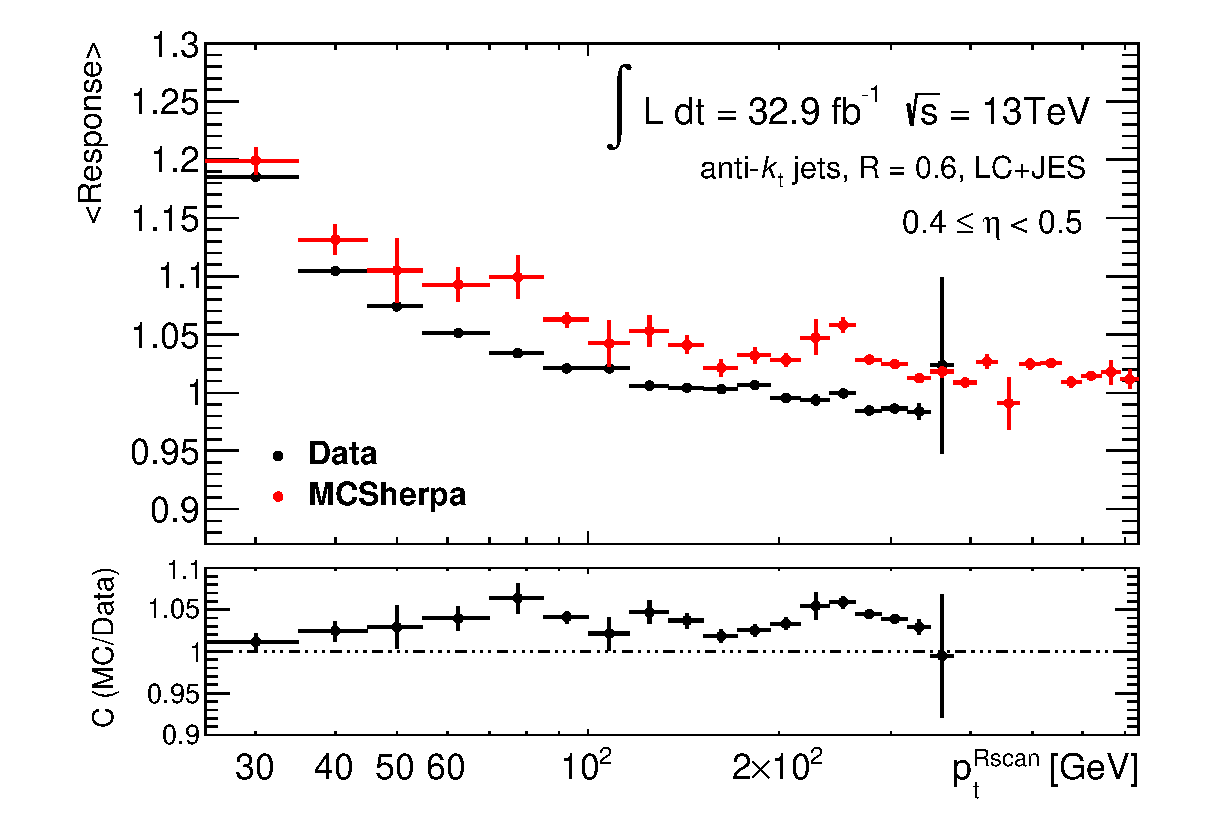
\includegraphics[width=\textwidth]{images/ResponseRatio6LC_49_Sherpa}
        \caption{$R=$0.6 ; 0.4$<\eta^{Rscan}_{det}<$0.5}
        %\label{fig:fitFeo}
    \end{subfigure}
    \hfill
    \begin{subfigure}[b]{0.495\textwidth}
        \centering
        \includegraphics[width=\textwidth]{images/ResponseRatio6LC_69_Sherpa}
        \caption{$R=$0.6 ; 2.4$<\eta^{Rscan}_{det}<$2.5}
        %\label{fig:Th26lc}
    \end{subfigure}
    \caption{ Paneles superiores: gráfico del valor medio $<\mathcal{R}>$ en función de $p_t^{Rscan}$ para datos (en negro) recolectados en ATLAS en 2016 y para la muestra de MC utilizada en el estudio de la incerteza sistemática asociada a la elección de simulación, generada utilizado Sherpa (en rojo). Paneles inferiores: cociente entre MC y Datos.} 
    \label{fig:ResponseSherpa}
\end{figure}

Para reducir el impacto de estas fluctuaciones y anular el de los ajustes malos, se utiliza una técnica de \textit{smoothing} sobre el cociente $\mathcal{C}$, obtenido luego de dividir $<\mathcal{R}>_{MC}$ por $<\mathcal{R}>_{Datos}$. El smoother se aplica en la dirección del momento, para cada bin de $\eta$. La idea del smoother es ajustar los puntos por un promedio pesado, que tiene en cuenta a los puntos vecinos, para obtener una descripción ``suave'' de la tendencia observada. Es decir, sobre un dado bin de $p_t$, el promedio se toma considerando todos los otros bines, donde sus respectivos pesos se asignan con un kernel Gaussiano que tiene en cuenta la distancia al bin considerado. Además, en dicho cálculo también se pesa cada bin por su error asociado.   

\begin{figure}[ht]
    \centering
    \begin{subfigure}[b]{0.495\textwidth}
        \centering
        \includegraphics[width=\textwidth]{images/Smo_2LC_pt_49.png}
        \caption{$R=$0.2 ; 0.4$<\eta^{Rscan}_{det}<$0.5}
        %\label{fig:data2lc49}
    \end{subfigure}
    \hfill
    \begin{subfigure}[b]{0.495\textwidth}
        \centering
        \includegraphics[width=\textwidth]{images/Smo_2LC_pt_69.png}
        \caption{$R=$0.2 ; 2.4$<\eta^{Rscan}_{det}<$2.5}
        %\label{fig:Th26lc}
    \end{subfigure}
    \vfill
    \begin{subfigure}[b]{0.495\textwidth}
        \centering
        \includegraphics[width=\textwidth]{images/Smo_6LC_pt_49.png}
        \caption{$R=$0.6 ; 0.4$<\eta^{Rscan}_{det}<$0.5}
        %\label{fig:fitFeo}
    \end{subfigure}
    \hfill
    \begin{subfigure}[b]{0.495\textwidth}
        \centering
        \includegraphics[width=\textwidth]{images/Smo_6LC_pt_69.png}
        \caption{$R=$0.6 ; 2.4$<\eta^{Rscan}_{det}<$2.5}
        %\label{fig:Th26lc}
    \end{subfigure}
    \caption{ En las figuras se muestra en rojo la corrección y en negro su valor suavizado (en el panel superior), y su cociente (en el panel inferior) en función de $p_t^{Rscan}$ obtenida a partir de datos recolectados en 2016 en ATLAS y usando la muestra nominal de MC, Powheg+Pythia. Las figuras superiores corresponden a la calibración derivada para Rscan Jets de $R=$0.2, y las inferiores para Rscan Jets de $R=$0.6. Las figuras de la izquierda representan un bin de $\eta$ central (0.4$<\eta^{Rscan}_{det}<$0.5) y las de la derecha uno más hacia el extremo del rango consideradp (2.4$<\eta^{Rscan}_{det}<$2.5)} 
    \label{fig:Smoothervspt}
\end{figure}

El uso del smoother debe realizarse con cuidado. La idea detrás de su uso es conseguir una calibración que sea independiente de las fluctuaciones estadísticas observadas. Para ello, se debe identificar una tendencia subyacente en los datos, de manera que la calibración no tenga en cuenta las fluctuaciones específicas de las muestras de estudio, y así cuando se aplique la calibración en otras muestras, no busque reproducirlas. Sin embargo, se debe tener presente que suavizar por demás puede deformar la calibración, perdiéndose la dependencia con el momento. Entonces, de cierta manera el criterio para decidir si el smoother es apropiado, es decir, si suaviza lo suficiente pero no demasiado, es un tanto arbitrario, pero completamente dependiente de la estadística con la que se trabaja. 

\begin{figure}[ht]
    \centering
    \begin{subfigure}[b]{0.495\textwidth}
        \centering
        \includegraphics[width=\textwidth]{images/Smo_2LC_ETA_1.png}
        \caption{$R=$0.2 ; 35GeV$<p_t^{Rscan}<$45GeV}
        %\label{fig:data2lc49}
    \end{subfigure}
    \hfill
    \begin{subfigure}[b]{0.495\textwidth}
        \centering
        \includegraphics[width=\textwidth]{images/Smo_2LC_ETA_2.png}
        \caption{$R=$0.2 ; 85GeV$<p^{Rscan}_t<$100GeV}
        %\label{fig:Th26lc}
    \end{subfigure}
    \vfill
    \begin{subfigure}[b]{0.495\textwidth}
        \centering
        \includegraphics[width=\textwidth]{images/Smo_6LC_ETA_1.png}
        \caption{$R=$0.6 ; 35GeV$<p_t^{Rscan}<$45GeV}
        %\label{fig:fitFeo}
    \end{subfigure}
    \hfill
    \begin{subfigure}[b]{0.495\textwidth}
        \centering
        \includegraphics[width=\textwidth]{images/Smo_6LC_ETA_2.png}
        \caption{$R=$0.6 ; 85GeV$<p^{Rscan}_t<$100GeV}
        %\label{fig:Th26lc}
    \end{subfigure}
    \caption{En las figuras se muestra en rojo la corrección y en negro su valor suavizado (en el panel superior), y su cociente (en el panel inferior) en función de $\eta^{Rscan}_{det}$ obtenida a partir de datos recolectados en 2016 en ATLAS y usando la muestra nominal de MC, Powheg+Pythia. Las figuras superiores corresponden a la calibración derivada para Rscan Jets de $R=$0.2, y las inferiores para Rscan Jets de $R=$0.6. Las figuras de la izquierda representan un bin de $p_t$ bajo (35GeV$<p_t^{Rscan}<$45GeV) y las de la derecha uno mayor (85GeV$<p^{Rscan}_t<$100GeV)} 
    \label{fig:SmoothervsEta}
\end{figure}

En la figura \ref{fig:Smoothervspt} se observa la corrección obtenida en función de $p_t^{Rscan}$ para ambas colecciones en dos bines de $\eta$ y los valores suavizados obtenidos. En el panel inferior de esta figura se observa el cociente entre ambos valores. Para ambos bines de $\eta$ y ambas colecciones se observa que la calibración suavizada sigue fielmente a la corrección derivada, salvo en los últimos bines de momento donde se observa que el cociente difiere de uno, indicando que se han efectivamente suavizado estos factores debido a que en estos puntos el error estadístico es mayor.   

En la figura \ref{fig:SmoothervsEta} se observan los factores de calibración obtenidos, y sus valores suavizados en función de $\eta_{det}$ para dos bines de momento. En esta figura se observa una simetría entre los $\eta$ positivos y los negativos, y una fuerte dependencia con $\eta$, como es de esperarse si se tiene en cuenta la geometría del detector. Se observa también que la corrección aumentará el momento de los Rscan Jets en los bines centrales de $\eta$, y, por el contrario, disminuirá su momento en los bines más externos. 
 
\begin{figure}[ht]
    \centering
    \begin{subfigure}[b]{0.495\textwidth}
        \centering
        \includegraphics[width=\textwidth]{images/Smo_2LC_pt_Sherpa_49.png}
        \caption{$R=$0.2 ; 0.4$<\eta^{Rscan}_{det}<$0.5}
        %\label{fig:data2lc49}
    \end{subfigure}
    \hfill
    \begin{subfigure}[b]{0.495\textwidth}
        \centering
        \includegraphics[width=\textwidth]{images/Smo_2LC_pt_Sherpa_69.png}
        \caption{$R=$0.2 ; 2.4$<\eta^{Rscan}_{det}<$2.5}
        \label{fig:fitMaloSherpa}
    \end{subfigure}
    \vfill
    \begin{subfigure}[b]{0.495\textwidth}
        \centering
        \includegraphics[width=\textwidth]{images/Smo_6LC_pt_49_Sherpa.png}
        \caption{$R=$0.6 ; 0.4$<\eta^{Rscan}_{det}<$0.5}
        %\label{fig:fitFeo}
    \end{subfigure}
    \hfill
    \begin{subfigure}[b]{0.495\textwidth}
        \centering
        \includegraphics[width=\textwidth]{images/Smo_6LC_pt_69_Sherpa.png}
        \caption{$R=$0.6 ; 2.4$<\eta^{Rscan}_{det}<$2.5}
        %\label{fig:Th26lc}
    \end{subfigure}
    \caption{  En las figuras se muestra en rojo la corrección y en negro su valor suavizado (en el panel superior), y su cociente (en el panel inferior) en función de $p_t^{Rscan}$ obtenida a partir de datos recolectados en 2016 en ATLAS y usando la muestra de MC generada en Sherpa para el estudio de la incerteza sistemática. Las figuras superiores corresponden a la calibración derivada para Rscan Jets de $R=$0.2, y las inferiores para Rscan Jets de $R=$0.6. Las figuras de la izquierda representan un bin de $\eta$ central (0.4$<\eta^{Rscan}_{det}<$0.5) y las de la derecha uno más hacia el extremo del rango considerado (2.4$<\eta^{Rscan}_{det}<$2.5).} 
    \label{fig:SmootherSherpa}
\end{figure}

En la figura \ref{fig:SmootherSherpa} se observa la corrección obtenida en función de $p_t$ para ambas colecciones en dos bines de $\eta$ y sus valores suavizados para el caso en que la muestra de MC utilizada fue la generada en Sherpa. En estas figuras se entiende con más claridad la necesidad de utilizar un smoother, ya que los puntos obtenidos presentan una mayor dispersión. En la mismas puede verse también como el método para suavizar beneficia aquellos puntos con menor error estadístico, reduce la influencia de aquellos con error un poco más significativo, y suprime el impacto de puntos como el que se observa en la figura \ref{fig:fitMaloSherpa}, producto de un ajusto malo. 

\begin{comment}
5- R-scan calibration
        - method
        - data and MC samples (paper 13TeV)
        - analysis
            - event selection: 
              - Basic Event Selection on GRID:
                - GRL / Flags / NPV / 
                - Primary Z selection
                  - Muon triggers, muon pt?
                  - weights?
                  - Cutflow: Size of data?
              - Event Cleaning: passLooseBad
              - Z + Jets Selection:
                - Z, muons overlap
                - RefJets & Rscan Jets
              - Isolation 
              - JVT
              - matching    
            - relative response
            - calibration
            - sistematic uncertainties
            - validation
            - comparison with dijet events
\end{comment}

Finalmente, las calibraciones obtenidas para ambas colecciones de jets se presentan, para dos bines de $\eta$ en la figura \ref{fig:FinalCalibration}, junto con su incerteza total, derivada según se explica en la sección \ref{Syst}.

%ctrl +shift + u3e
%ctrl +shift + u3c
\chapter{Validación}\label{Validation}

Una vez obtenida la calibración para la colección de Rscan jets se busca comprobar que no queden diferencias residuales entre MC y datos. Para ver esto, se estudia nuevamente el cociente $\mathcal{C}$ presentado en la sección \ref{Rscan} siguiendo el mismo proceso tanto en la selección de eventos como en los cortes cinemáticos, con la salvedad de que ahora los Rscan Jets, únicamente en datos, se encuentran calibrados, además, con la calibración in-situ derivada en \ref{Derivandow}. La calibración, suavizada, está representada por un histograma bidimensional, bineado tanto en $\eta^{Rscan}_{det}$ como en $p_t^{Rscan}$. Para aplicarla, se identifican el $p_t$ y el $\eta$ del Rscan Jet que se quiere calibrar, y se interpola bi-linealmente el histograma de la calibración en este punto, obteniéndose así el factor de corrección multiplicativo a aplicar al momento del Rscan Jet. 

Una vez calibrados los Rscan Jets, se procede de la misma manera en la construcción de los gráficos de $<\mathcal{R}>$. Se espera que ahora que los datos han sido corregidos, el cociente $\mathcal{C}$, que representa la diferencia entre datos y MC, sea uno. En la figura \ref{fig:Closure} se puede ver la response obtenida en datos a partir de los Rscan Jets calibrados con esta nueva corrección in-situ en función de $p_t$ y para dos bines de $\eta$ y ambas colecciones de Rscan Jets, y el cociente $\mathcal{C}$ calculado entre $<\mathcal{R}>_{MC}$ y $<\mathcal{R}>_{datos+InsituCorr}$. Se puede ver que la diferencia residual entre datos y MC luego de aplicada la calibración es $\leq 1\%$ en los rangos de momento mostrados. En general, para los bines de $\eta$ estudiados se observa buen acuerdo (tolerancia =$1\%$) en todo el rango de momento en el que se tiene una calibración: para los Rscan Jets con $R=$0.2 (0.6), este rango es $p_t>$15GeV (25GeV) y $p_t\sim$200GeV, llegando hasta $p_t=290$GeV (300GeV) en la región $|\eta|<$0.8 y a $p_t=$150GeV en el rango 2.5$<|\eta|<$3.


%https://en.wikipedia.org/wiki/Bilinear_interpolation

\begin{figure}[ht]
    \centering
    \begin{subfigure}[b]{0.495\textwidth}
        \centering
        \includegraphics[width=\textwidth]{images/Closure2LC_49}
        \caption{$R=$0.2 ; 0.4$<\eta^{Rscan}_{det}<$0.5}
        %\label{fig:data2lc49}
    \end{subfigure}
    \hfill
    \begin{subfigure}[b]{0.495\textwidth}
        \centering
        \includegraphics[width=\textwidth]{images/Closure2LC_69}
        \caption{$R=$0.2 ; 2.4$<\eta^{Rscan}_{det}<$2.5}
        %\label{fig:Th26lc}
    \end{subfigure}
    \vfill
    \begin{subfigure}[b]{0.495\textwidth}
        \centering
        \includegraphics[width=\textwidth]{images/Closure6LC_49}
        \caption{$R=$0.6 ; 0.4$<\eta^{Rscan}_{det}<$0.5}
        %\label{fig:fitFeo}
    \end{subfigure}
    \hfill
    \begin{subfigure}[b]{0.495\textwidth}
        \centering
        \includegraphics[width=\textwidth]{images/Closure6LC_69}
        \caption{$R=$0.6 ; 2.4$<\eta^{Rscan}_{det}<$2.5}
        %\label{fig:Th26lc}
    \end{subfigure}
    \caption{ En las figuras se muestra en rojo la response en la muestra nominal de MC, Powheg+Pythia, tal y como se construyó en la sección \ref{Derivandow}. En negro, se muestra la response de los datos construida ahora con Rscan Jets cuyo momento ha sido corregido por la calibración derivada en \ref{Derivandow}. En los paneles superiores se muestran $<\mathcal{R}>$, en función de $p_t^{Rscan}$, luego de atravesar el mismo proceso de selección de eventos y recortes cinemáticos que al derivarse la calibración. En los paneles inferiores se muestra el cociente entre $<\mathcal{R}>_{MC}$ y $<\mathcal{R}>_{Datos+InsituCorr}$. Las líneas punteadas representan la región de ancho de 2$\%$ de diferencia entre datos y MC.}
    \label{fig:Closure}
\end{figure}


%There are small deviations visible, but they are randomly distributed and they correspond to points with large uncertainties.
\chapter{Estudio (preliminar) de las Incertezas Sistemáticas}\label{Syst}

La elección de algunos valores al momento de realizar selecciones de eventos es, de cierta manera, arbitraria. Si bien, por ejemplo, la decisión del umbral tanto para el criterio de aislación como para el matching está motivada por argumentos de geometría, no deja de ser una elección. Por lo tanto, se debe estudiar el impacto de realizar variaciones sobre estos parámetros en la calibración derivada, obteniéndose así las incertezas sistemáticas de este método. Un resumen de las incertezas sistemáticas estudiadas en esta tesis se presenta en la tabla \ref{tab:syst}


\begin{table}[ht]
    \centering
    \begin{tabular}{|l|l|l|} 
        \hline
        %\multicolumn{2}{|c|}{input} & \multicolumn{2}{c|}{output} & \\
        Sistemático & Descripción & Variación \\ \hline\hline
        \textbf{Muones} & &\\
        Escala & Incerteza en la escala de energía de los muones & $\pm 1\sigma$\\
        Resolución (ID) &  Incerteza en la resolución del momento de los & $\pm 1\sigma$\\
        & en el ID & \\ \hline
        \textbf{Método de} & &\\
        \textbf{Direct-Matching} &  &\\ 
        JES & Incerteza en la escala de energía de los Ref. Jets & $\pm 1\sigma$\\ 
        JVT & Incerteza en la discriminación de pile-up jets & 0.11 $(\downarrow)$ 0.91 $(\uparrow)$ \\
        Jets aislados ($f$) & $\Delta R> f*R$ & $f=$ 1.5$(\downarrow)$, 2.5$(\uparrow)$ \\
        $p_{t,\%}$ & relación de momento en aislación de jets & 5$\%(\downarrow)$ $20\%(\uparrow)$ \\
        Matching ($dR$) & $\Delta R(jet^{Rscan},jet^{Ref})<dR$ & $dR=$ 0.1$(\downarrow)$, 0.3$(\uparrow)$ \\ \hline 
        \textbf{Generador de MC}& Diferencia entre generadores de MC & Sherpa \\ \hline 
        \end{tabular}
    \caption{Resumen de incertezas sistemáticas estudiadas para las calibraciones R-scan en eventos de $Z+jets$.}
    \label{tab:syst}
\end{table}


En este trabajo, se estudiaron variaciones sistemáticas sobre los parámetros mencionados en la tabla \ref{tab:syst}, a valores por encima y por debajo del utilizado en la derivación de la calibración. Estos parámetros están directamente relacionados con el método utilizado, el método de direct-matching. Para el caso del parámetro JVT, las variaciones propuestas en la tabla \ref{tab:syst} corresponden a $\pm 1\sigma$ en la discriminación de pile-up jets y surgen de recomendaciones dadas en la ref. \cite{JVTtool}. 

Además de los sistemáticos asociados a cortes cinemáticos, se tienen que tener cuenta sistemáticos heredados de pasos anteriores a la aplicación del método de direct-matching, por ejemplo, incertezas asociadas a la identificación y corrección del momento de los muones. Estas variaciones también se corresponden a variaciones de $\pm 1\sigma$ según las recomendaciones dadas por el grupo CP de ATLAS en la ref. \cite{MCPGuidelines}. 

La elección del MC es otro factor que debe estudiarse. Como se mencionó en la sección \ref{predictions}, distintos generadores de MC (o combinaciones de ellos) simulan los eventos de maneras diferentes desde el elemento de matriz considerado, o el orden de la predicción, hasta el modelado del pile-up, el evento subyacente, las PDFs, la fragmentación y la hadronización. Entonces, con el fin de estudiar qué pasaría si se hubiera derivado la calibración con otra muestra de MC, en este trabajo se introduce una segunda muestra generada en Sherpa según se especifica en la sección \ref{Muestras}. 

Para todas las variaciones mencionadas arriba, el procedimiento utilizado para derivar las incertezas sistemáticas fue el mismo. Para cada parámetro se proponen dos variaciones, una por encima y una por debajo del valor utilizado; y para cada variación se vuelve a derivar una corrección tal y como se explica en la sección \ref{Derivandow}, manteniendo las otras fijas en el valor nominal.

En el caso de la elección de MC, se cuenta con una sola muestra extra a parte de la nominal. En particular, como ya se discutió en la sección \ref{Derivandow}, la muestra de Sherpa resultó tener poca estadística por lo que la corrección derivada con la misma presenta muchas fluctuaciones sustanciales.

Una vez obtenidas las correcciones a partir de estos parámetros variados, se las suaviza, y para cada bin de $p_t$ se calcula la diferencia relativa entre la corrección ``variada'' y la nominal. Una aclaración, quizás evidente, es que una variación de un parámetro  a un valor por encima del nominal no necesariamente se traduce en una variación de la corrección monótonamente hacia arriba, o hacia abajo, sino que la calibración correspondiente a la variación por encima de un dado parámetro puede encontrarse para algunos bines de momento por encima de la nominal y para otros por debajo. Por este motivo, y con el fin de simetrizar la incerteza a derivar, se guarda como contribución del parámetro, la diferencia relativa (al nominal) máxima, en valor absoluto, de las dos variaciones. 

En este punto se incorpora también una incerteza asociada a la calibración de los Ref Jets. Ésta es la incerteza de la JES estudiada en la referencia \cite{JESpaper}, que se corresponde con la incerteza total en la cadena completa de calibración para jets reconstruidos con el algoritmo anti-k$_t$ $R=$0.4 a partir de la escala EM. Esta incerteza fue proporcionada por el grupo de JetEtmiss de ATLAS.

La incerteza sistemática (relativa) total se obtiene de sumar las contribuciones de cada parámetro en cuadratura para cada bin de $\eta$ y $p_t$. 
En la figura \ref{fig:Un} se observa la incerteza sistemática (relativa) total (en negro), en función del momento transverso del jet, y las contribuciones de cada parámetro estudiado a la misma, para dos bines de $\eta$ y para ambas colecciones de Rscan Jets. De la misma se observa que la contribución más significativa es la incerteza de las JES en primera medida, y la asociada a la elección del MC. Las incertezas asociadas a la identificación y  corrección de momento de los muones, y la de JVT son insignificantes (menores al 0.4$\%$) frente a la contribución de la JES, la cual alcanza el 5$\%$ a bajo momento y decrece hasta el 2$\%$ hacia el extremo del rango de momento considerado. En las figuras \ref{fig:Un} (b) y (d) correspondientes al bin 2.4$<\eta^{Rscan}_{det}<$2.5 el hecho de que las curvas se vuelvan chatas en los últimos bines de momento no es representativo de la incerteza, sino de que en esos bines no se cuenta con calibración. 
La incerteza sistemática (relativa) total es del orden del 5$\%$ por debajo de los 30 GeV, y disminuye al 2$\%$ al llegar a los 200GeV.


\begin{figure}[ht]
    \centering
    \begin{subfigure}[b]{0.495\textwidth}
        \centering
        \includegraphics[width=\textwidth]{images/SumIn2_Eta_49_2LC_wContributions.eps}
        \caption{$R=$0.2 ; 0.4$<\eta^{Rscan}_{det}<$0.5}
        %\label{fig:data2lc49}
    \end{subfigure}
    \hfill
    \begin{subfigure}[b]{0.495\textwidth}
        \centering
        \includegraphics[width=\textwidth]{images/SumIn2_Eta_69_2LC_wContributions.eps}
        \caption{$R=$0.2 ; 2.4$<\eta^{Rscan}_{det}<$2.5}
        %\label{fig:Th26lc}
    \end{subfigure}
    \vfill
    \begin{subfigure}[b]{0.495\textwidth}
        \centering
        \includegraphics[width=\textwidth]{images/SumIn2_Eta_49_6LC_wContributions.eps}
        \caption{$R=$0.6 ; 0.4$<\eta^{Rscan}_{det}<$0.5}
        %\label{fig:fitFeo}
    \end{subfigure}
    \hfill
    \begin{subfigure}[b]{0.495\textwidth}
        \centering
        \includegraphics[width=\textwidth]{images/SumIn2_Eta_69_6LC_wContributions.eps}
        \caption{$R=$0.6 ; 2.4$<\eta^{Rscan}_{det}<$2.5}
        %\label{fig:Th26lc}
    \end{subfigure}
    \caption{ Incerteza Sistemática relativa total, en negro, y sus distintas contribuciones en función de $p_t^{Rscan}$, en bines de 0.4$<\eta^{Rscan}_{det}<$0.5 a la izquierda y de 2.4$<\eta^{Rscan}_{det}<$2.5 a la derecha. Las figuras de arriba corresponden a la colección de Rscan Jets con $R=$0.2 y las de abajo con 0.6. } 
    \label{fig:Un}
\end{figure}


\begin{figure}[ht]
    \centering
    \begin{subfigure}[b]{0.495\textwidth}
        \centering
        \includegraphics[width=\textwidth]{images/SumIn2_pT_4_2LC_wContributions.eps}
        \caption{$R=$0.2 ; 45GeV$<p_t^{Rscan}<$55GeV}
        %\label{fig:data2lc49}
    \end{subfigure}
    \hfill
    \begin{subfigure}[b]{0.495\textwidth}
        \centering
        \includegraphics[width=\textwidth]{images/SumIn2_pT_10_2LC_wContributions.eps}
        \caption{$R=$0.2 ; 134GeV$<p^{Rscan}_t<$152GeV}
        %\label{fig:Th26lc}
    \end{subfigure}
    \vfill
    \begin{subfigure}[b]{0.495\textwidth}
        \centering
        \includegraphics[width=\textwidth]{images/SumIn2_pT_4_6LC_wContributions.eps}
        \caption{$R=$0.6 ; 45GeV$<p_t^{Rscan}<$55GeV}
        %\label{fig:fitFeo}
    \end{subfigure}
    \hfill
    \begin{subfigure}[b]{0.495\textwidth}
        \centering
        \includegraphics[width=\textwidth]{images/SumIn2_pT_10_6LC_wContributions.eps}
        \caption{$R=$0.6 ; 134GeV$<p^{Rscan}_t<$152GeV}
        %\label{fig:Th26lc}
    \end{subfigure}
    \caption{ Incerteza sistemática relativa total (en negro), y sus contribuciones, en función de $\eta_{det}$ en el bin de 45GeV$<p_t^{Rscan}<$55GeV a la derecha, y 134GeV$<p^{Rscan}_t<$152GeV a la izquierda. Las figuras superiores corresponden a la coelcción de Rscan Jets con $R=$0.2 y las inferiores a 0.6.} 
    \label{fig:UnvsEta}
\end{figure}

En la figura \ref{fig:UnvsEta} se observa la incerteza sistemática (relativa) total (en negro), en función $\eta_{det}$, y las contribuciones de cada parámetro estudiado a la misma, para dos bines de $p_t$ y para ambas colecciones de Rscan Jets. Nuevamente, se hace evidente en estas figuras que la contribución más significativa es la incerteza de las JES. Las incertezas correspondientes a las demás contribuciones muestran una gran variabilidad en la dirección de $\eta$. Dejando de lado esas fluctuaciones del orden del 1$\%$, se observa que la dependencia con $\eta$ de la incerteza total se hereda directamente de la contribución de la JES; y la misma es poco dependiente, manteniéndose del orden de alrededor del 4$\%$ a bajo momento, y más dependiente a alto momento, de casi un 3$\%$ en los bines de $\eta$ extremos y disminuyendo hasta el 1$\%$ hacia los bines centrales.\\


Finalmente, se presentan las calibraciones R-scan obtenidas en este trabajo para dos bines de $\eta$ en la figura \ref{fig:FinalCalibration}. Junto al factor de corrección se muestra la incerteza estadística y la incerteza total en función de $p_t^{Rscan}$.



\begin{figure}[ht]
    \centering
    \begin{subfigure}[b]{0.495\textwidth}
        \centering
        \includegraphics[width=\textwidth]{images/Final2LC/Calibration_Eta_49.eps}
        \caption{$R=$0.2 ; 0.4$<\eta^{Rscan}_{det}<$0.5}
        %\label{fig:data2lc49}
    \end{subfigure}
    \hfill
    \begin{subfigure}[b]{0.495\textwidth}
        \centering
        \includegraphics[width=\textwidth]{images/Final2LC/Calibration_Eta_69.eps}
        \caption{$R=$0.2 ; 2.4$<\eta^{Rscan}_{det}<$2.5}
        %\label{fig:Th26lc}
    \end{subfigure}
    \vfill
    \begin{subfigure}[b]{0.495\textwidth}
        \centering
        \includegraphics[width=\textwidth]{images/Final6LC/Calibration_Eta_49.eps}
        \caption{$R=$0.6 ; 0.4$<\eta^{Rscan}_{det}<$0.5}
        %\label{fig:fitFeo}
    \end{subfigure}
    \hfill
    \begin{subfigure}[b]{0.495\textwidth}
        \centering
        \includegraphics[width=\textwidth]{images/Final6LC/Calibration_Eta_69.eps}
        \caption{$R=$0.6 ; 2.4$<\eta^{Rscan}_{det}<$2.5}
        %\label{fig:Th26lc}
    \end{subfigure}
    \caption{ Calibración R-scan obtenida para Rscan Jets con $R=$ 0.2, (a) y (b) y 0.6 (c) y (d), en función de $p_t^{Rscan}$. Las figuras de la derecha corresponden al bin 2.4$<\eta^{Rscan}_{det}<$2.5 y las de la izquierda al bin 0.4$<\eta^{Rscan}_{det}<$0.5. En negro se muestra el calibración (suavizada); en celeste se muestra la incerteza total (suma en cuadratura de la componente estadística y la incerteza sistemática); y en azul más oscuro, la componente estadística de la incerteza.} 
    \label{fig:FinalCalibration}
\end{figure}



\afterpage{\null\newpage}
\chapter{Comparación con Eventos de Dijets}\label{dijets}

Dentro del grupo de Física Experimental de Altas Energías del DF\footnote{Departamento de Física, FCEyN, UBA}, actualmente se está realizando un trabajo similar en torno a calibraciones R-scan, pero utilizando una selección de eventos de dijets.

Una vez realizada la selección de eventos correspondiente, se aplica el mismo método de direct-matching como fue explicado en la sección \ref{Rscan}. La ventaja de esta selección de eventos es que permite obtener una calibración al momento de Rscan Jets en un rango de momento más extendido, por ejemplo, alcanzando un momento de $p_t\sim$1TeV con una incerteza estadística del orden del 0.2$\%$ en los bines de $\eta$ centrales. Sin embargo, ésta no permite ir hacia valores de momento bajo: por debajo de $p_t<$100GeV la incerteza estadística asociada aumenta hasta el 1$\%$, y hasta el 2$\%$ por debajo de los 60GeV. Si bien este trabajo actualmente continúa en curso, en la figura \ref{fig:Comparison} se pueden ver resultados preliminares de dicho estudio con eventos de dijets para el caso de Rscan Jets con $R=$0.6. La incerteza sistemática que se muestra en la figura se corresponde a contribuciones de los parámetros del método de direct-matching: JVT, aislación ($f$) y matching ($dR$) (ver tabla \ref{tab:sel}) tomando los mismos valores para sus respectivas variaciones; y a la contribución de la elección del generador de MC. A esta incerteza sistemática, se le incorporó además la incerteza asociada a la JES, que es la misma que la aplicada en el caso de eventos de $Z+jets$. 

En la figura \ref{fig:Comparison} también se muestra la calibración derivada en esta tesis, junto con su incerteza total con el fin de comparar las calibraciones en el rango de momento en el que se solapan. De estas figuras queda claro como se distribuye la estadística para una selección de eventos y para la otra. Mientras que para el caso de $Z$+$jets$ se logra derivar una corrección para $p_t>$25GeV con una banda de error estadístico de ancho $<$1$\%$ hasta un $p_t\sim$100GeV, y aumentando  hasta un ancho de $\sim1$.5$\%$ en $p_t\sim300$GeV; para el caso de dijets se observa un comportamiento opuesto, con una componente estadística, en general, de ancho $>2\%$ y en algunos casos, como el de la figura \ref{fig:stat}, de ancho mayor al 8$\%$ a bajo momento, que disminuye hasta una ancho de 0.5$\%$ llegando a 1TeV. 

Ambas calibraciones comparten el rango de momento entre 45Gev$<p_t<$300GeV. En las figuras (a), (b) y (c) puede verse que en un primer tramo de este intervalo las bandas estadísticas de ambas calibraciones se solapan, mientras que en el resto del intervalo se observa que la superposición se da gracias a la contribución de las incertezas sistemáticas a la incerteza total. 

Si bien ambas selecciones de eventos se usan para derivar una calibración en dos rangos distintos pero que se superponen, no necesariamente debiera una ser, en algún sentido, ``continuación'' de la otra. Esta sospecha se encuentra relacionada con el hecho de que la selección de eventos de dijets, discrimina eventos de naturaleza QCD mientras que la de $Z$+$jets$ prioriza eventos de tipo semi-leptónicos.



\begin{figure}[ht]
    \centering
    \begin{subfigure}[b]{0.495\textwidth}
        \centering
        \includegraphics[width=\textwidth]{images/ComparisonW_dijets_Eta_45.eps}
        \caption{0.0$<\eta^{Rscan}_{det}<$0.1}
        %\label{fig:data2lc49}
    \end{subfigure}
    \hfill
    \begin{subfigure}[b]{0.495\textwidth}
        \centering
        \includegraphics[width=\textwidth]{images/ComparisonW_dijets_Eta_49.eps}
        \caption{ 0.4$<\eta^{Rscan}_{det}<$0.5}
        %\label{fig:Th26lc}
    \end{subfigure}
    \vfill
    \begin{subfigure}[b]{0.495\textwidth}
        \centering
        \includegraphics[width=\textwidth]{images/ComparisonW_dijets_Eta_54.eps}
        \caption{0.9$<\eta^{Rscan}_{det}<$1.0}
        \label{fig:stat}
    \end{subfigure}
    \hfill
    \begin{subfigure}[b]{0.495\textwidth}
        \centering
        \includegraphics[width=\textwidth]{images/ComparisonW_dijets_Eta_69.eps}
        \caption{2.4$<\eta^{Rscan}_{det}<$2.5}
        %\label{fig:Th26lc}
    \end{subfigure}
    \caption{ Comparación entre la calibración Rscan derivada para Rscan Jets de radio 0.6 en eventos de $Z+jets$ (en rojo) y en eventos de dijets (en azul) para distintos bines de $\eta$. Para cada calibración se muestra también la incerteza total y su componente estadística.} 
    \label{fig:Comparison}
\end{figure}










\chapter{Conclusiones}\label{Conclus}

El proceso estándar de calibración de jets es uno que ocupa gran cantidad de tiempo y esfuerzo humano dentro del experimento ATLAS. El hecho de que la última calibración oficial\cite{JESpaper} de ATLAS derivada para jets reconstruidos con $R=$0.4 haya demorado alrededor de dos años en publicarse es motivo suficiente para afirmar que no es factible producir una calibración para cada radio de interés. 

Esto representa un obstáculo para los diferentes estudios que allí se llevan a cabo. Por ejemplo, distintas mediciones de precisión de SM reclaman una calibración para jets de radio 0.6 para reducir el impacto de las incertezas causadas por radiación que cae fuera del cono del jet cuando este es reconstruido con un radio 0.4. Otro ejemplo que se puede mencionar son los estudios de física boosteada donde se requiere una calibración para jets de radio 0.2 para poder analizar la subestructura de jets que engloban a los decaimientos de una partícula boosteada. Este tipo de física está presente en muchas búsquedas \textit{beyond-SM}.  

Una solución a la creciente demanda de las mismas es el método de R-scan. Este es un método sencillo, de tipo in-situ, que propone calibrar jets de tamaño $R$ respecto de jets reconstruidos y calibrados de manera estándar. 

En el marco de esta tesis, y utilizando los datos de colisiones $pp$ a $\sqrt{s}=$13TeV recolectados por el detector ATLAS en 2016, se derivaron dos calibraciones Rscan, una para $R=$0.2 y otra para $R=$0.6, junto con sus correspondientes incertezas. Además, se realizó una validación de las mismas al aplicárselas a los Rscan jets en datos y concluir que no se observan diferencias residuales (con una tolerancia del $1\%$) entre datos y MC. Finalmente, se realizó una comparación en la que la calibración para $R=$0.6 derivada en eventos de $Z+jets$ en este trabajo resultó ser consistente con otra calibración Rscan derivada en eventos de muchos jets en el rango de momento transverso en el que se solapan.     






\clearpage
\bibliographystyle{ieeetr}
\makebibliography


\begin{comment}
\begin{appendices}
\include{appendices/appendix1}
\end{appendices}
\end{comment}
\end{document}


\begin{comment}
1- Introduction
2- Theoretical Overview
    - The Standard Model
        - brevemente: sectores
        - limitaciones (?)
        - QCD: confinement and asymtotic freedom
    - Physics at hadron colliders
        - Jets
3- The LHC and the ATLAS experiment (hablar de pile up en algun momento)
4- Jets 
    - jet algos
    - jet inputs
    - jet reconstruction (paper 13TeV) and default calibration
 
6- Conclusions
\end{comment}